\documentclass[french]{beamer}
\usepackage{babel}
\usepackage[utf8x]{inputenc}
\usepackage[babel=true]{csquotes}
\usepackage{hyperref}
\usepackage[footheight=1em]{beamerthemeboxes}
%\usepackage{pgfpages}
%\setbeameroption{show notes on second screen=left}
\usetheme{Singapore}

%\usetheme{Frankfurt}


%\addfootboxtemplate{\color{white}}{\color{gray}
  %\insertframenumber/\inserttotalframenumber\null}



%\setbeamertemplate{background canvas}{\includegraphics
%   [width=\paperwidth,height=\paperheight]{img/fond.png}}


\title{
\includegraphics[width=0.3\textwidth]{img/logo_cogito} \\ Intelligence Artificielle :\\une approche cognitive }
\subtitle{\textit{\footnotesize Travail d'Étude et de Recherche \\ Master Informatique 1$^{\grave{e}re}$ année (GMIN20B)}}
\author{William Dyce \and Thibaut Marmin \\ Namrata Patel \and Clément Sipieter}
\institute{Université Montpellier 2\\Encadré par Violaine Prince et Guillaume Tisserant}
\date{7 mai 2012}

\begin{document}

\AtBeginSection[]
{
  \begin{frame}{
\includegraphics[width=0.3\textwidth]{img/logo_cogito}}{Analyse et implémentation d'un modèle de conscience artificielle}
  \begin{columns}[t]
  \begin{column}{5cm}
  \tableofcontents[sections={1-3},currentsection,hideothersubsections]
  \end{column}
  \begin{column}{5cm}
  \tableofcontents[sections={4-6},currentsection,hideothersubsections]
  \end{column}
  \end{columns}
  \end{frame}
}

\begin{frame}
\titlepage
\end{frame}

\begin{frame}{
\includegraphics[width=0.3\textwidth]{img/logo_cogito}}{Analyse et implémentation d'un modèle de conscience artificielle}
    

  \begin{columns}[t]
  \begin{column}{5cm}
  \tableofcontents[sections={1-3},hideallsubsections]
  \end{column}
  \begin{column}{5cm}
  \tableofcontents[sections={4-6},hideallsubsections]
  \end{column}
  \end{columns}

\end{frame}

\section{Introduction}
\subsection{Rappel historique}
%----------------------------------------
% RAPPEL HISTORIQUE - DEEP BLUE
%----------------------------------------

\begin{frame}{Rappel historique}{Deep Blue}

\begin{block}{Deep Blue} 
\begin{itemize}
\item Victoire contre Garry Kasparov en 1997.
\item $1^{\grave{e}re}$ défaite de grand maître sous contraintes normales de temps.
\end{itemize}
\end{block}

\pause

\begin{block}{R. Levinson} 
\begin{itemize}
\item \textit{\og But doesn't know that it's playing chess.\fg{}}
\item Intelligence? Artificielle? Synthétique?
\end{itemize}
\end{block}

\end{frame}



%----------------------------------------
% RAPPEL HISTORIQUE - THÉORIE DES JEUX
%----------------------------------------

\begin{frame}{Rappel historique}{Théorie des Jeux}

\begin{block}{Théorème du Minimax} 
\begin{itemize}
\item J. Von Neumann, 1928.
\item \textit{Stratégie optimale pour un joueur donné.}
\end{itemize}
\end{block}

\pause

\begin{block}{Équilibre de Nash} 
\begin{itemize}
\item J. F. Nash, 1950.
\item \textit{Union de stratégies, localement optimale pour tous.}
\end{itemize}
\end{block}

\end{frame}


%----------------------------------------
% RAPPEL HISTORIQUE - LIMITES
%----------------------------------------

\begin{frame}{Rappel historique}{Limites}

\begin{block}{Domaine d'application}
\begin{itemize}
\item \underline{Minimax}: Jeux compétitifs, à deux joueurs, à somme nulle.
\item \underline{Minimax \& Nash}: Durée et nombre d'options finis.
\end{itemize}
\end{block}

\pause

\begin{block}{Temps de calcul}
\begin{itemize}
\item Complexité moyenne \emph{$O(b^{\frac{d}{2}})$} si trié et élagé:
	\begin{itemize}
	\item d : longeur de la partie.
	\item b : nombre d'options par tour.
	\end{itemize}
\item En pratique: besoin d'heuristiques, donc perte d'optimalité.
\end{itemize}
\end{block}

\end{frame}

\subsection{Projet de recherche}
\begin{frame}{Présentation du sujet}
	\begin{itemize}
		\item Intelligence artificielle
		\pause
		\item Approche différente d'un projet
		\pause
		\item Rêve de l'IA
	\end{itemize}
\end{frame}

\begin{frame}{Présentation du sujet}{Une approche cognitive}
	\begin{itemize}
		\item Apprentissage
		\item Reconnaissance de formes
		\item Classification
		\item Polyvalence du système
	\end{itemize}
\end{frame}


\subsection{Un modèle de conscience artificielle}
\begin{frame}{Un modèle de conscience artificielle}{Origine du modèle}
\begin{itemize}
  \item ``Consicence
  artificielle'' par Guillaume Tisserant, Guillaume Travail du module
  'Cognition' du M2 en 2010
  \item Modèle de représentation proposé dans le Chapitre 4.
\end{itemize}
\end{frame}

\begin{frame}{Un modèle de conscience artificielle}{Version simplifiée du
modèle}
\begin{center}
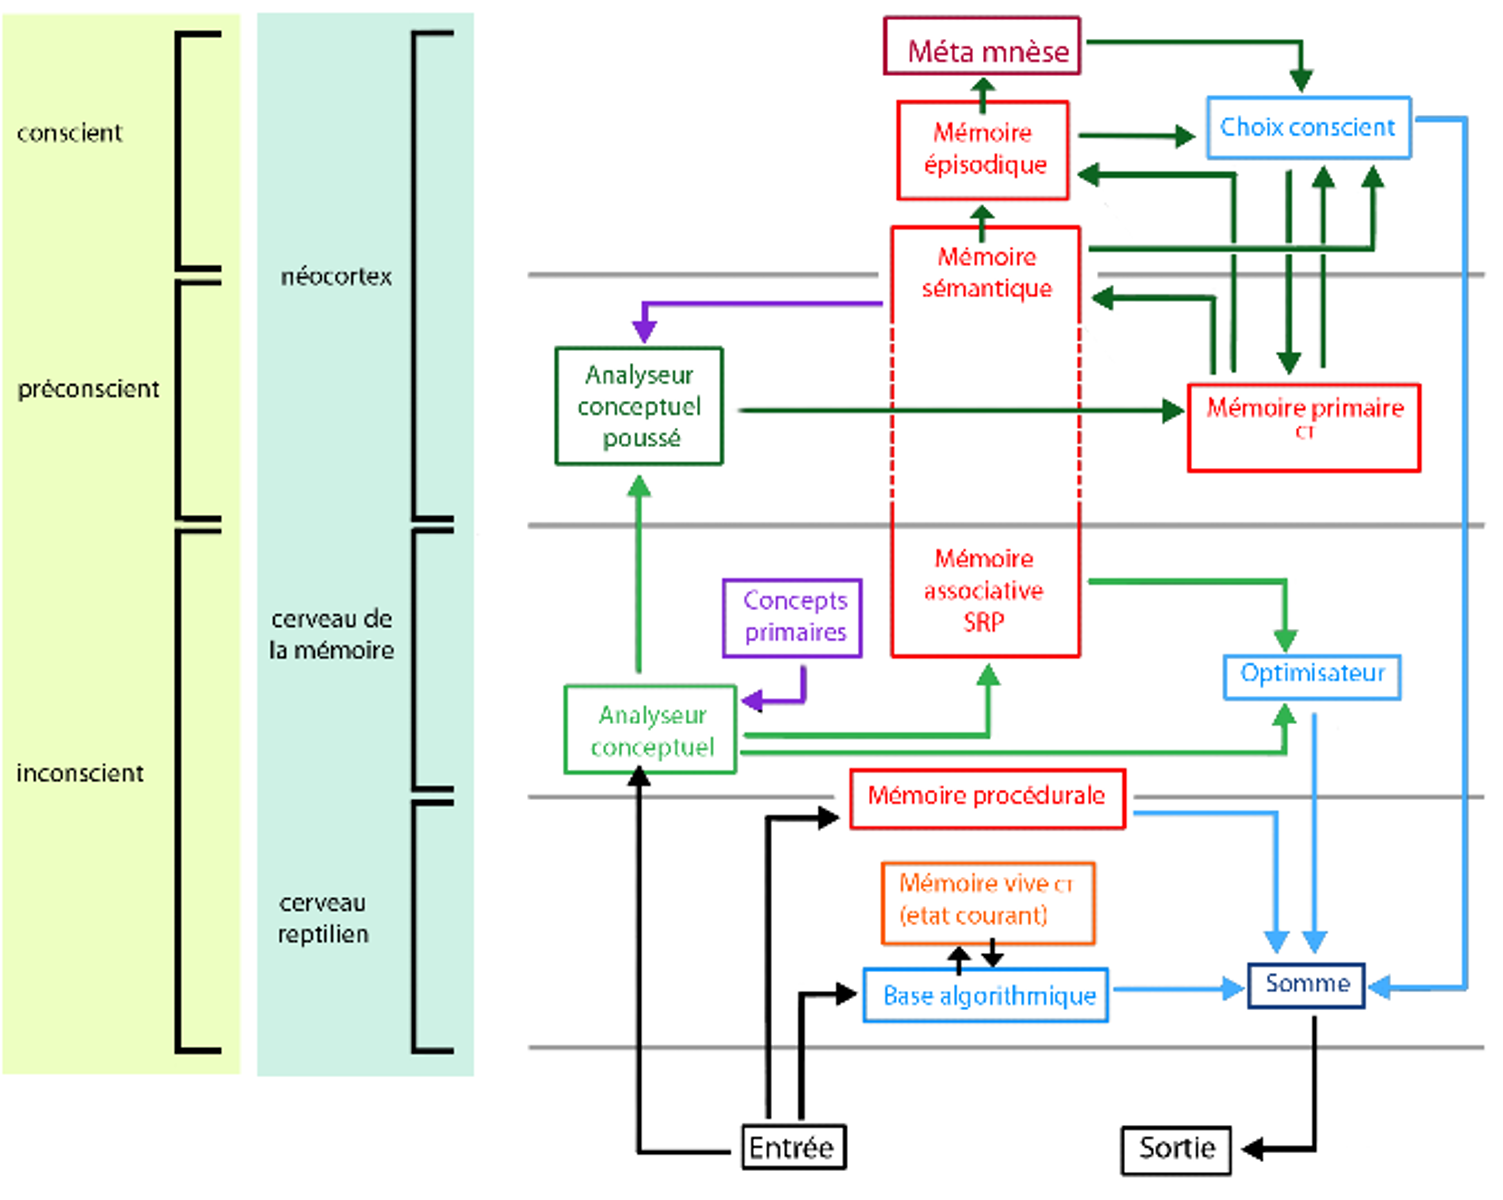
\includegraphics[width=0.9\textwidth]{img/intro/modele_original}
\end{center}
\end{frame}



\section{Analyse Générale}
\subsection{Contraintes de réalisation}
\begin{frame}{Contraintes de réalisation}{Temporelle , d'effectifs et de
compétences}
\begin{itemize}
  \item Temps : travail à réaliser en trois mois
  \item Effectif : quatre membres dans l'équipe
  \item Compétences :
  \begin{itemize}
    \item Compétences requises à la \textbf {fin} du semestre \newline =
    Compétences nécessaires pour la réalisation du projet
    \item Cours données souvent trop tard pour assurer leur bonne application au
    projet
  \end{itemize}
\end{itemize}
\end{frame}


\subsection{Restrictions appliquées au modèle}
\begin{frame}{Restrictions appliquées au modèle}{Environnement , fonctionnement}
\begin{tabular}{l l}
\begin{minipage}{0.6\textwidth}\begin{center}
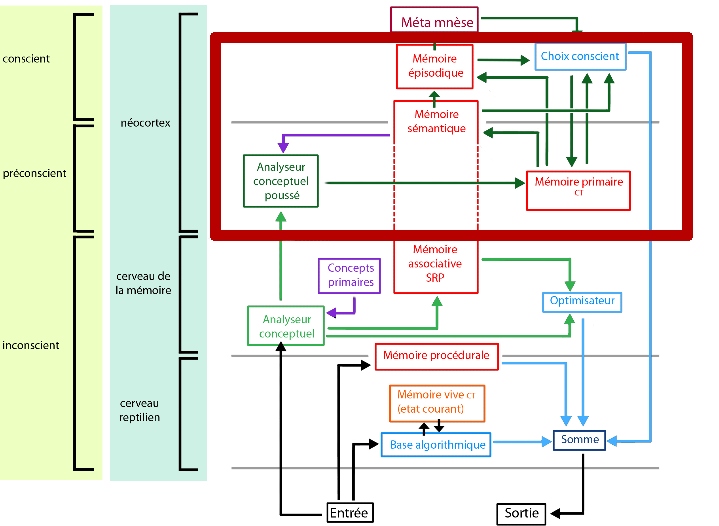
\includegraphics[width=\textwidth]{img/analyse_generale/modele_restraint}
\end{center}\end{minipage} & \begin{minipage}{0.4\textwidth}
\begin{itemize}
  \item \textbf{Environnement : }Limitation à un type précis de jeu
  \item \textbf{Fonctionnement : }Retrait et simulation des parties
  \begin{itemize}
    \item Retrait de la métamnèse
    \item Simulation de la partie inconsciente
  \end{itemize}
\end{itemize}
\end{minipage}
\end{tabular}
\end{frame}


\subsection{Domaine d'application}
%----------------------------------------
% DOMAINE D'APPLICATION : POUQUOI
%----------------------------------------
\begin{frame}{Domaine d'application}{Jeu de plateau}

\begin{block}{Pourquoi le jeu de plateau ?}
\begin{itemize}
\item Convergence \texttt{DECOL} / \texttt{IMAGINA}.
\pause
\item Activité purement cognitive.
\pause
\item Activité cognitive complète.
\pause
\item Évaluation facile de la performance.
\end{itemize}
\end{block}

\end{frame}


%----------------------------------------
% LE MINIMAX
%----------------------------------------
\begin{frame}{Domaine d'application}{Théorie des jeux}

\begin{block}{Théorème du MiniMax}
\begin{itemize}
\item J. Von Neumann, 1928.
\item \textit{Stratégie optimale pour un joueur donné.}
\end{itemize}
\end{block}
\end{frame}


%----------------------------------------
% LIMITES DU MINIMAX
%----------------------------------------

\begin{frame}{Domaine d'application}{Limites du MiniMax}

\begin{block}{Type de confrontation}
\begin{itemize}
\item \underline{Minimax}: Jeux compétitifs, à deux joueurs, à somme nulle.
\item \underline{Minimax \& Nash}: Durée et nombre d'options finis.
\end{itemize}
\end{block}

\pause

\begin{block}{Temps de calcul}
\begin{itemize}
\item En moyenne \emph{$O(b^{\frac{d}{2}})$} :
	\begin{itemize}
	\item d : longeur partie.
	\item b : options par tour.
	\end{itemize}
\item En pratique : besoin d'heuristiques $\Rightarrow$ perte d'optimalité.
\end{itemize}
\end{block}

\end{frame}

\section{Analyse \& Implémentation}
\subsection{Environnement \& simulation}
%----------------------------------------
% ARCHITECTURE GLOBALE
%----------------------------------------
\begin{frame}{Environnement}{Architecture Globale}
\begin{center}
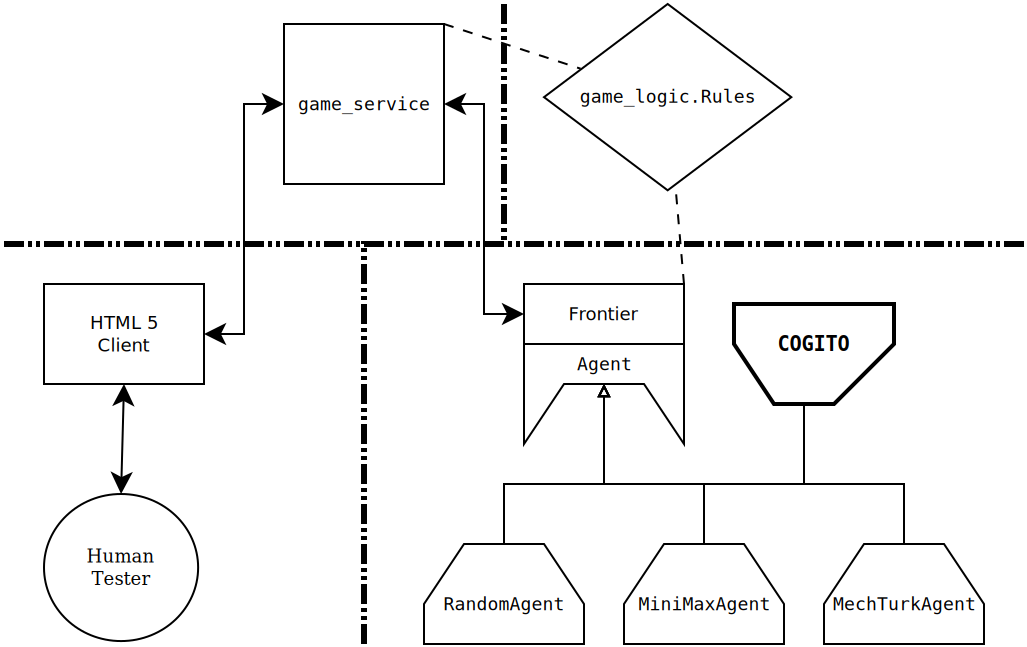
\includegraphics[width=0.8\textwidth]{img/william/archi_full}\\
\end{center}
\end{frame}
%----------------------------------------
% DÉCOUPLAGE AGENT-ENVIRONEMENT
%----------------------------------------
\begin{frame}{Environnement}{Découplage}
\begin{itemize}
\item Modèle \og Black Board \fg{}
\item Communication \og Stigmergique \fg{}
\end{itemize}
\begin{center}
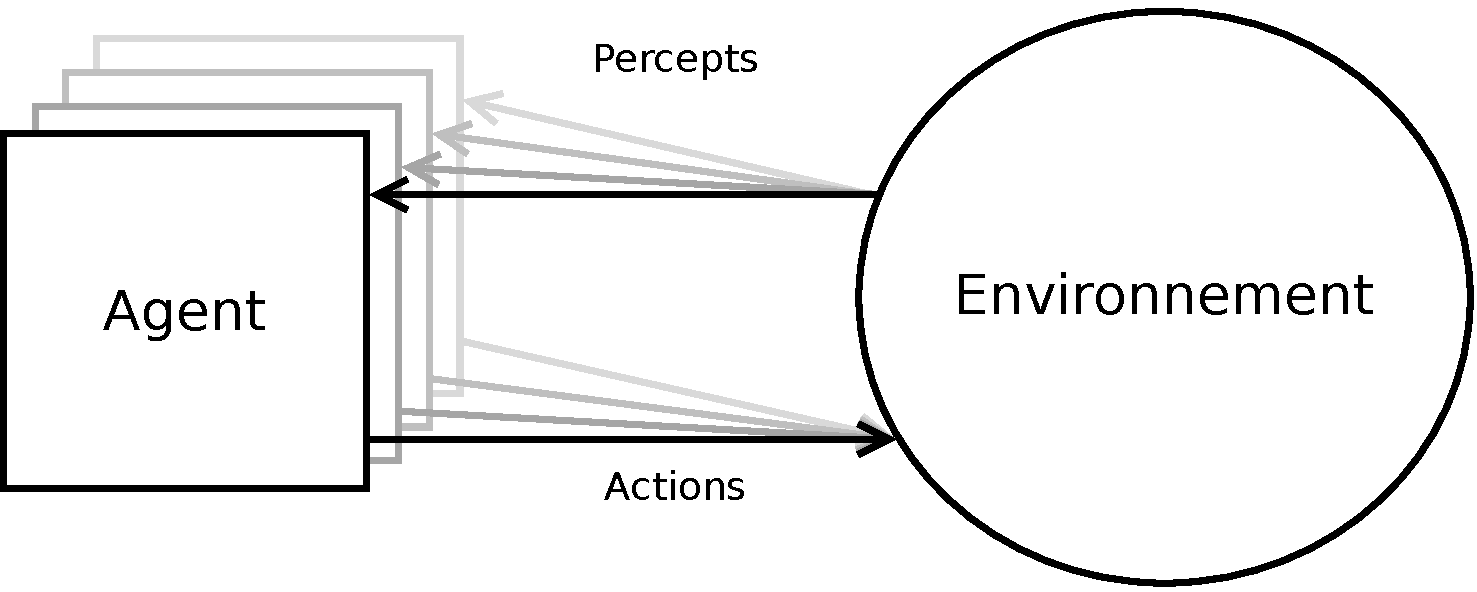
\includegraphics[width=0.8\textwidth]{img/william/agent_env}\\
\end{center}
\end{frame}
%----------------------------------------
% ARBITRE
%----------------------------------------
%\begin{frame}{Environnement}{Arbitre}
%\begin{center}
%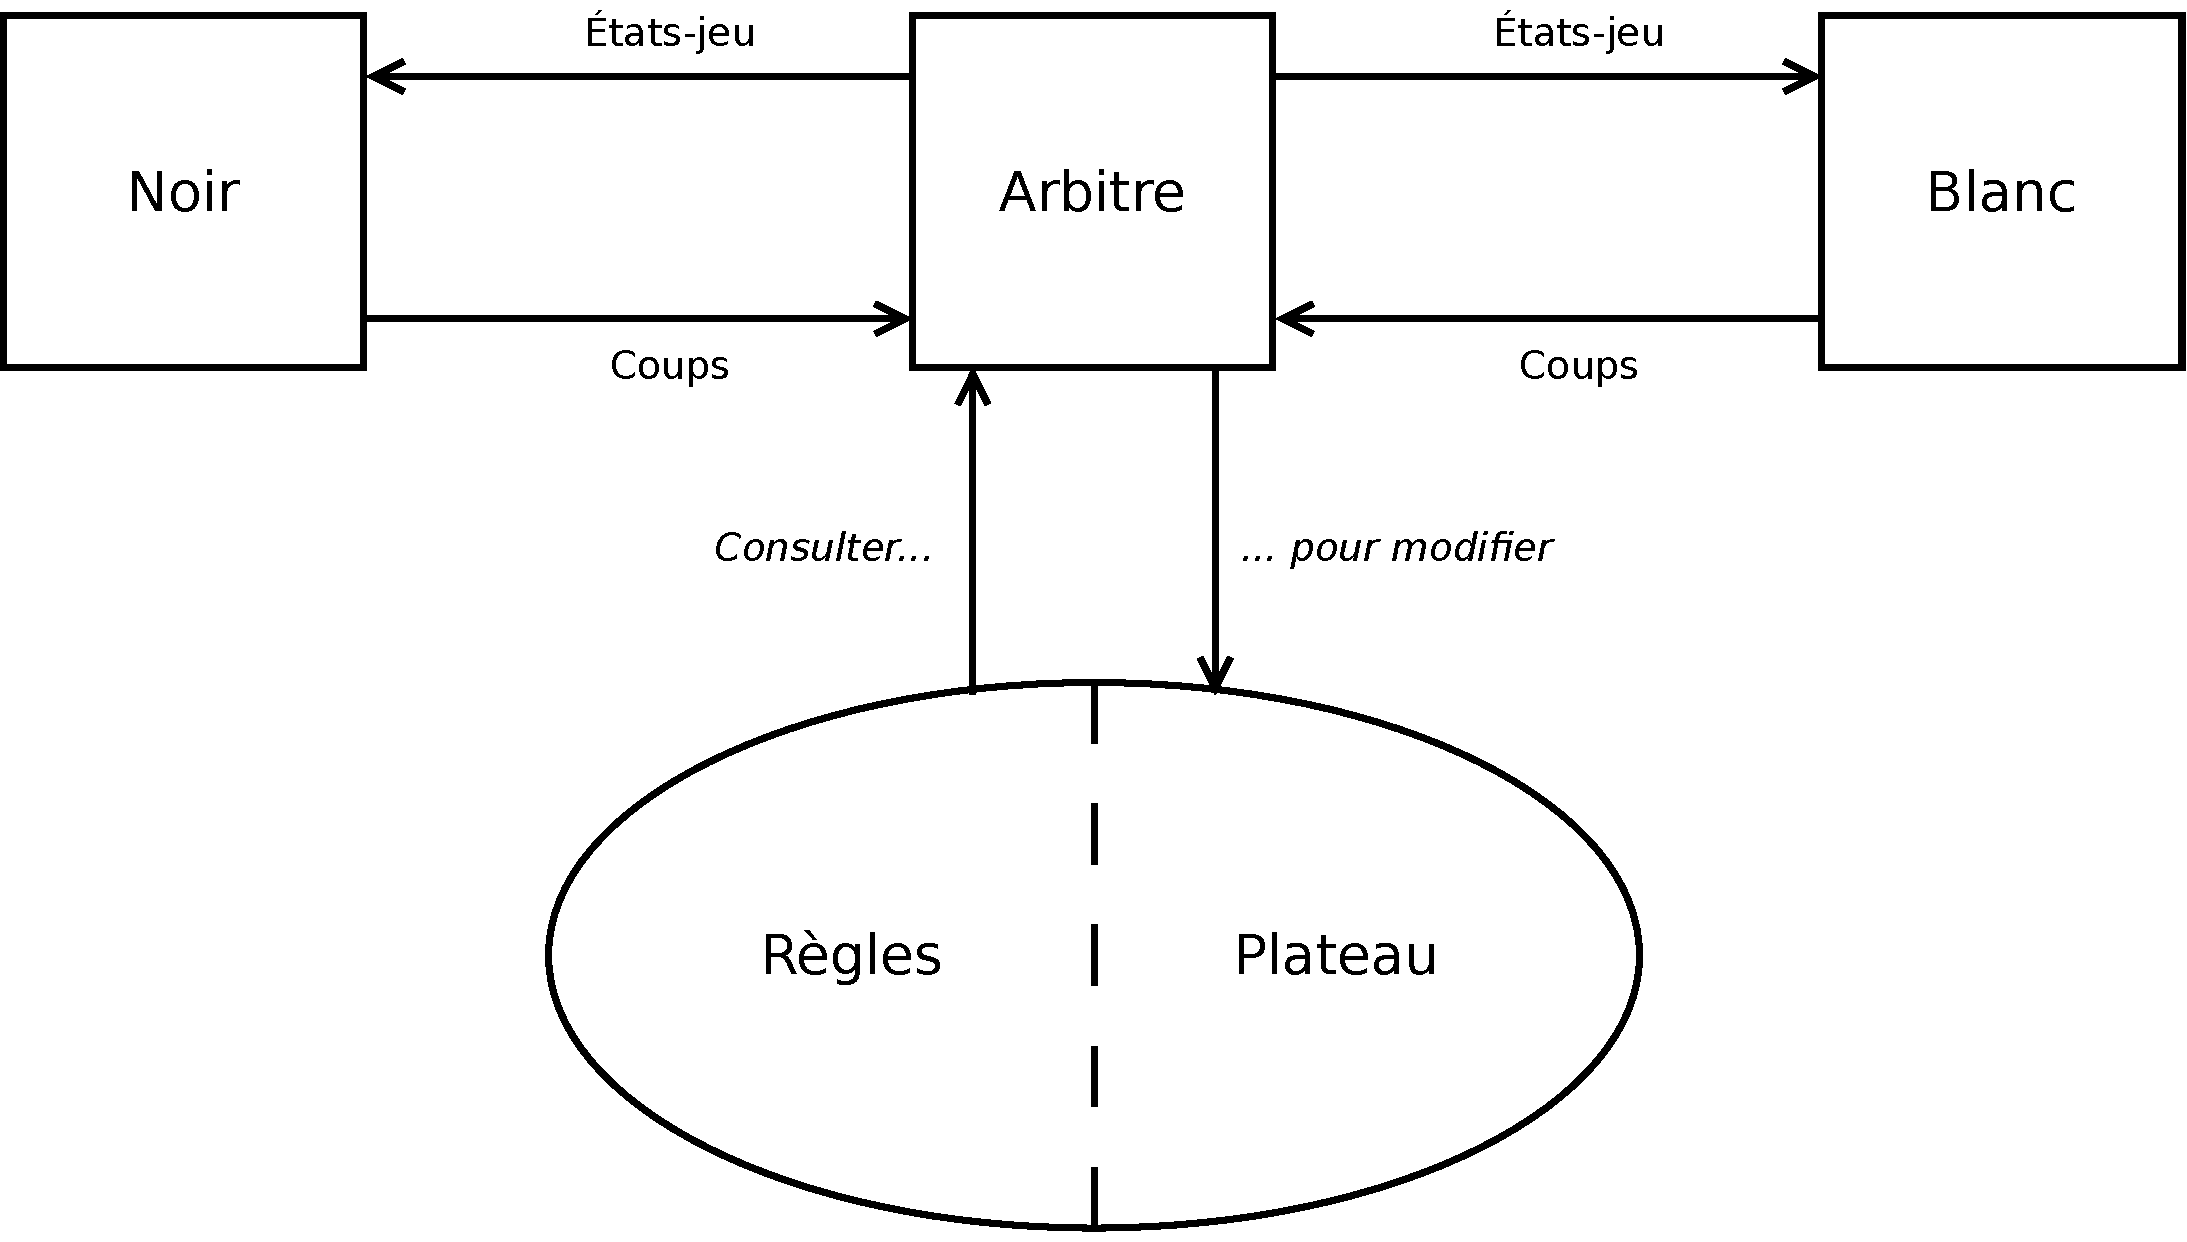
\includegraphics[width=\textwidth]{img/william/arbitre}\\
%\end{center}
%\end{frame}
%----------------------------------------
% ARHITECTURE CLIENT-SERVEUR
%----------------------------------------
\begin{frame}{Environnement}{Architecture client-serveur}
\begin{center}
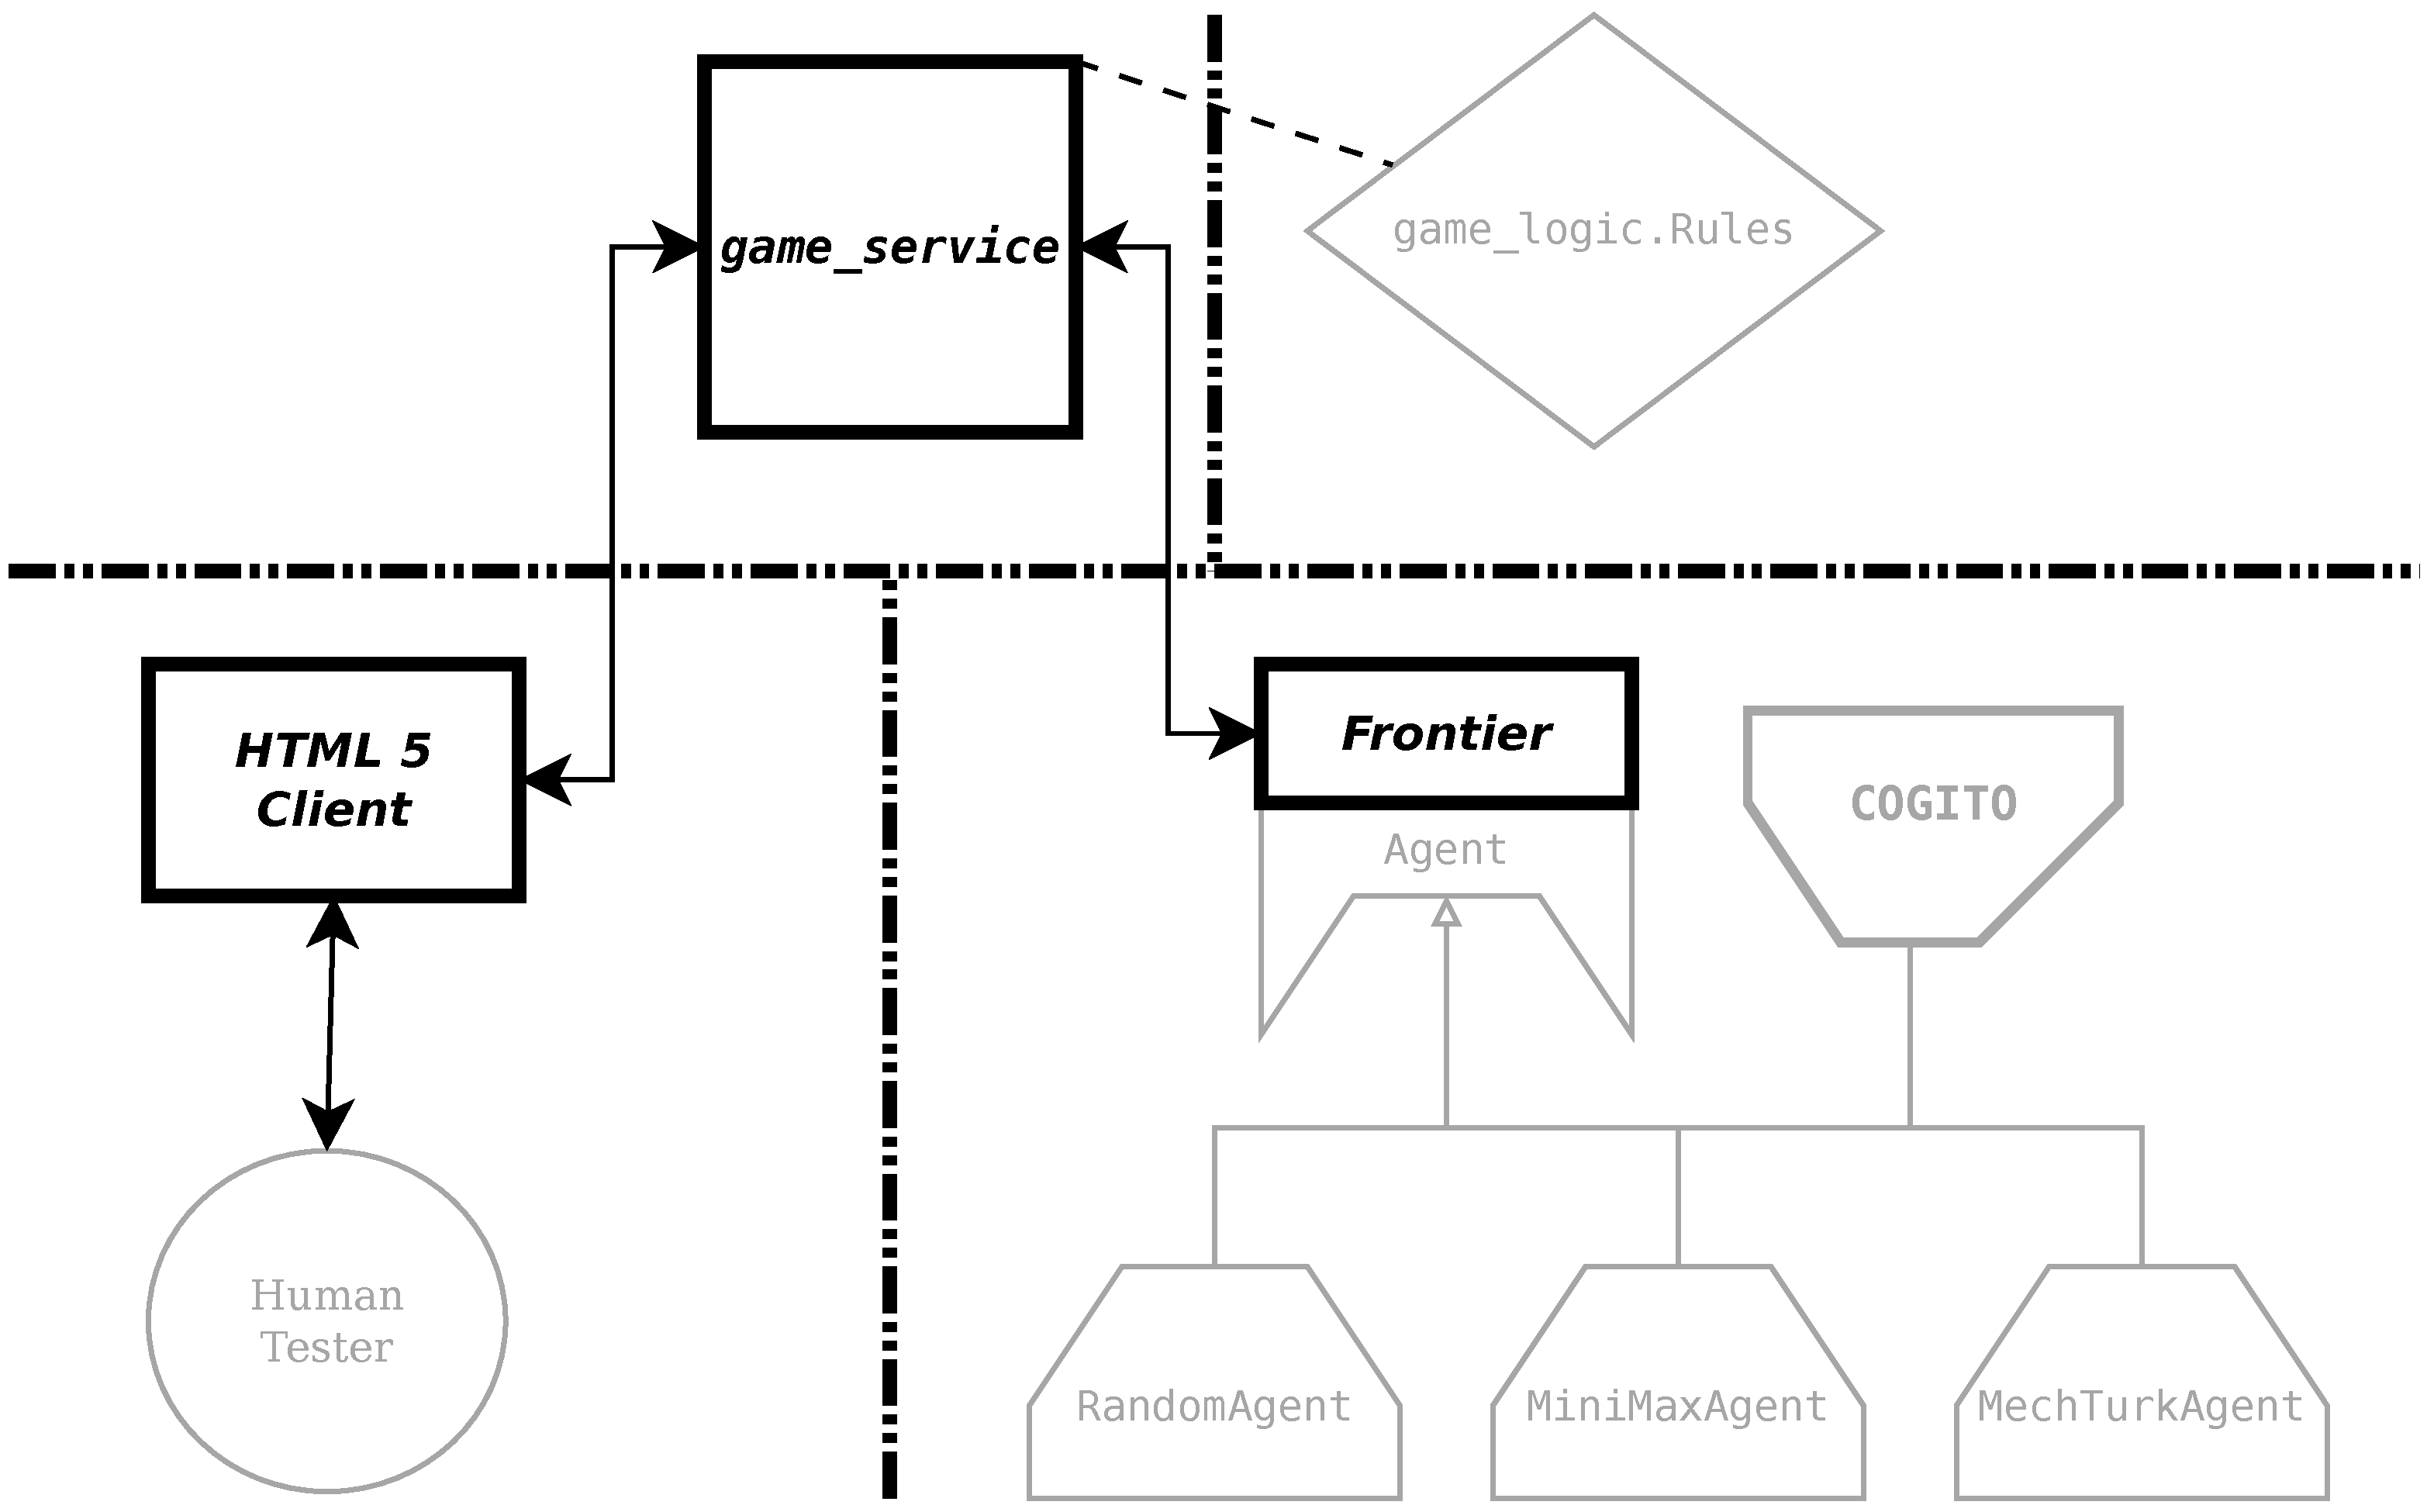
\includegraphics[width=0.8\textwidth]{img/william/archi_clients_serveur}\\
\end{center}
\end{frame}
%----------------------------------------
% GAME_LOGIC -- SHARED
%----------------------------------------
\begin{frame}{Environnement}{Redondance}
Besoin d'une ressource commune :
\begin{center}
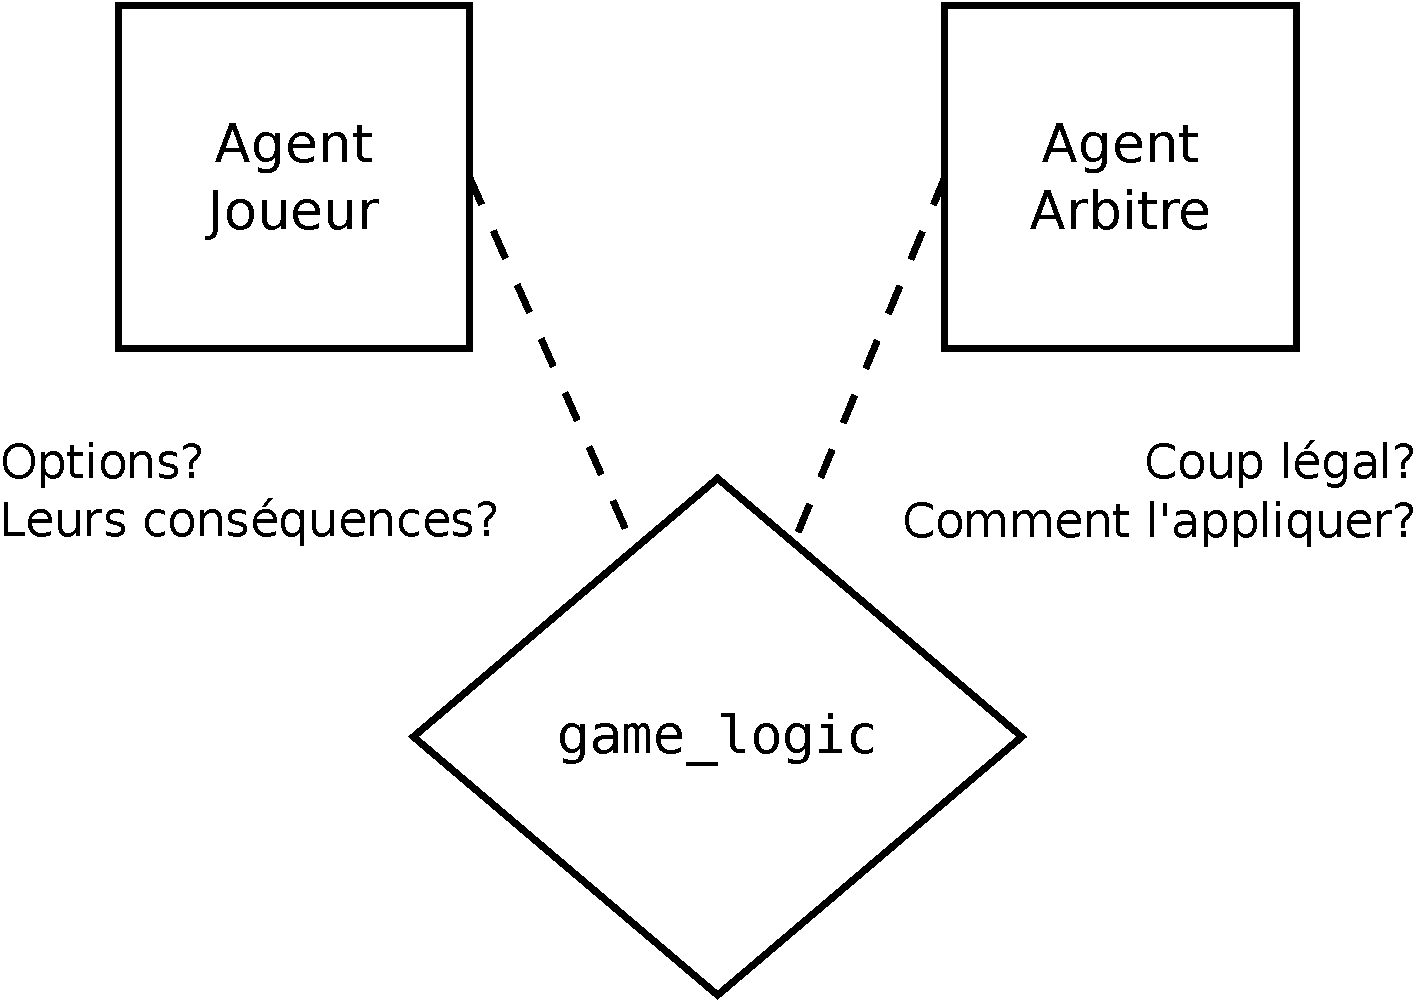
\includegraphics[width=0.6\textwidth]{img/william/game_logic_shared}\\
\end{center}
\end{frame}
%----------------------------------------
% GAME_LOGIC -- VUE GLOBALE
%----------------------------------------
\begin{frame}{Environnement}{Bibliothèque \texttt{game\_logic}}
\begin{center}
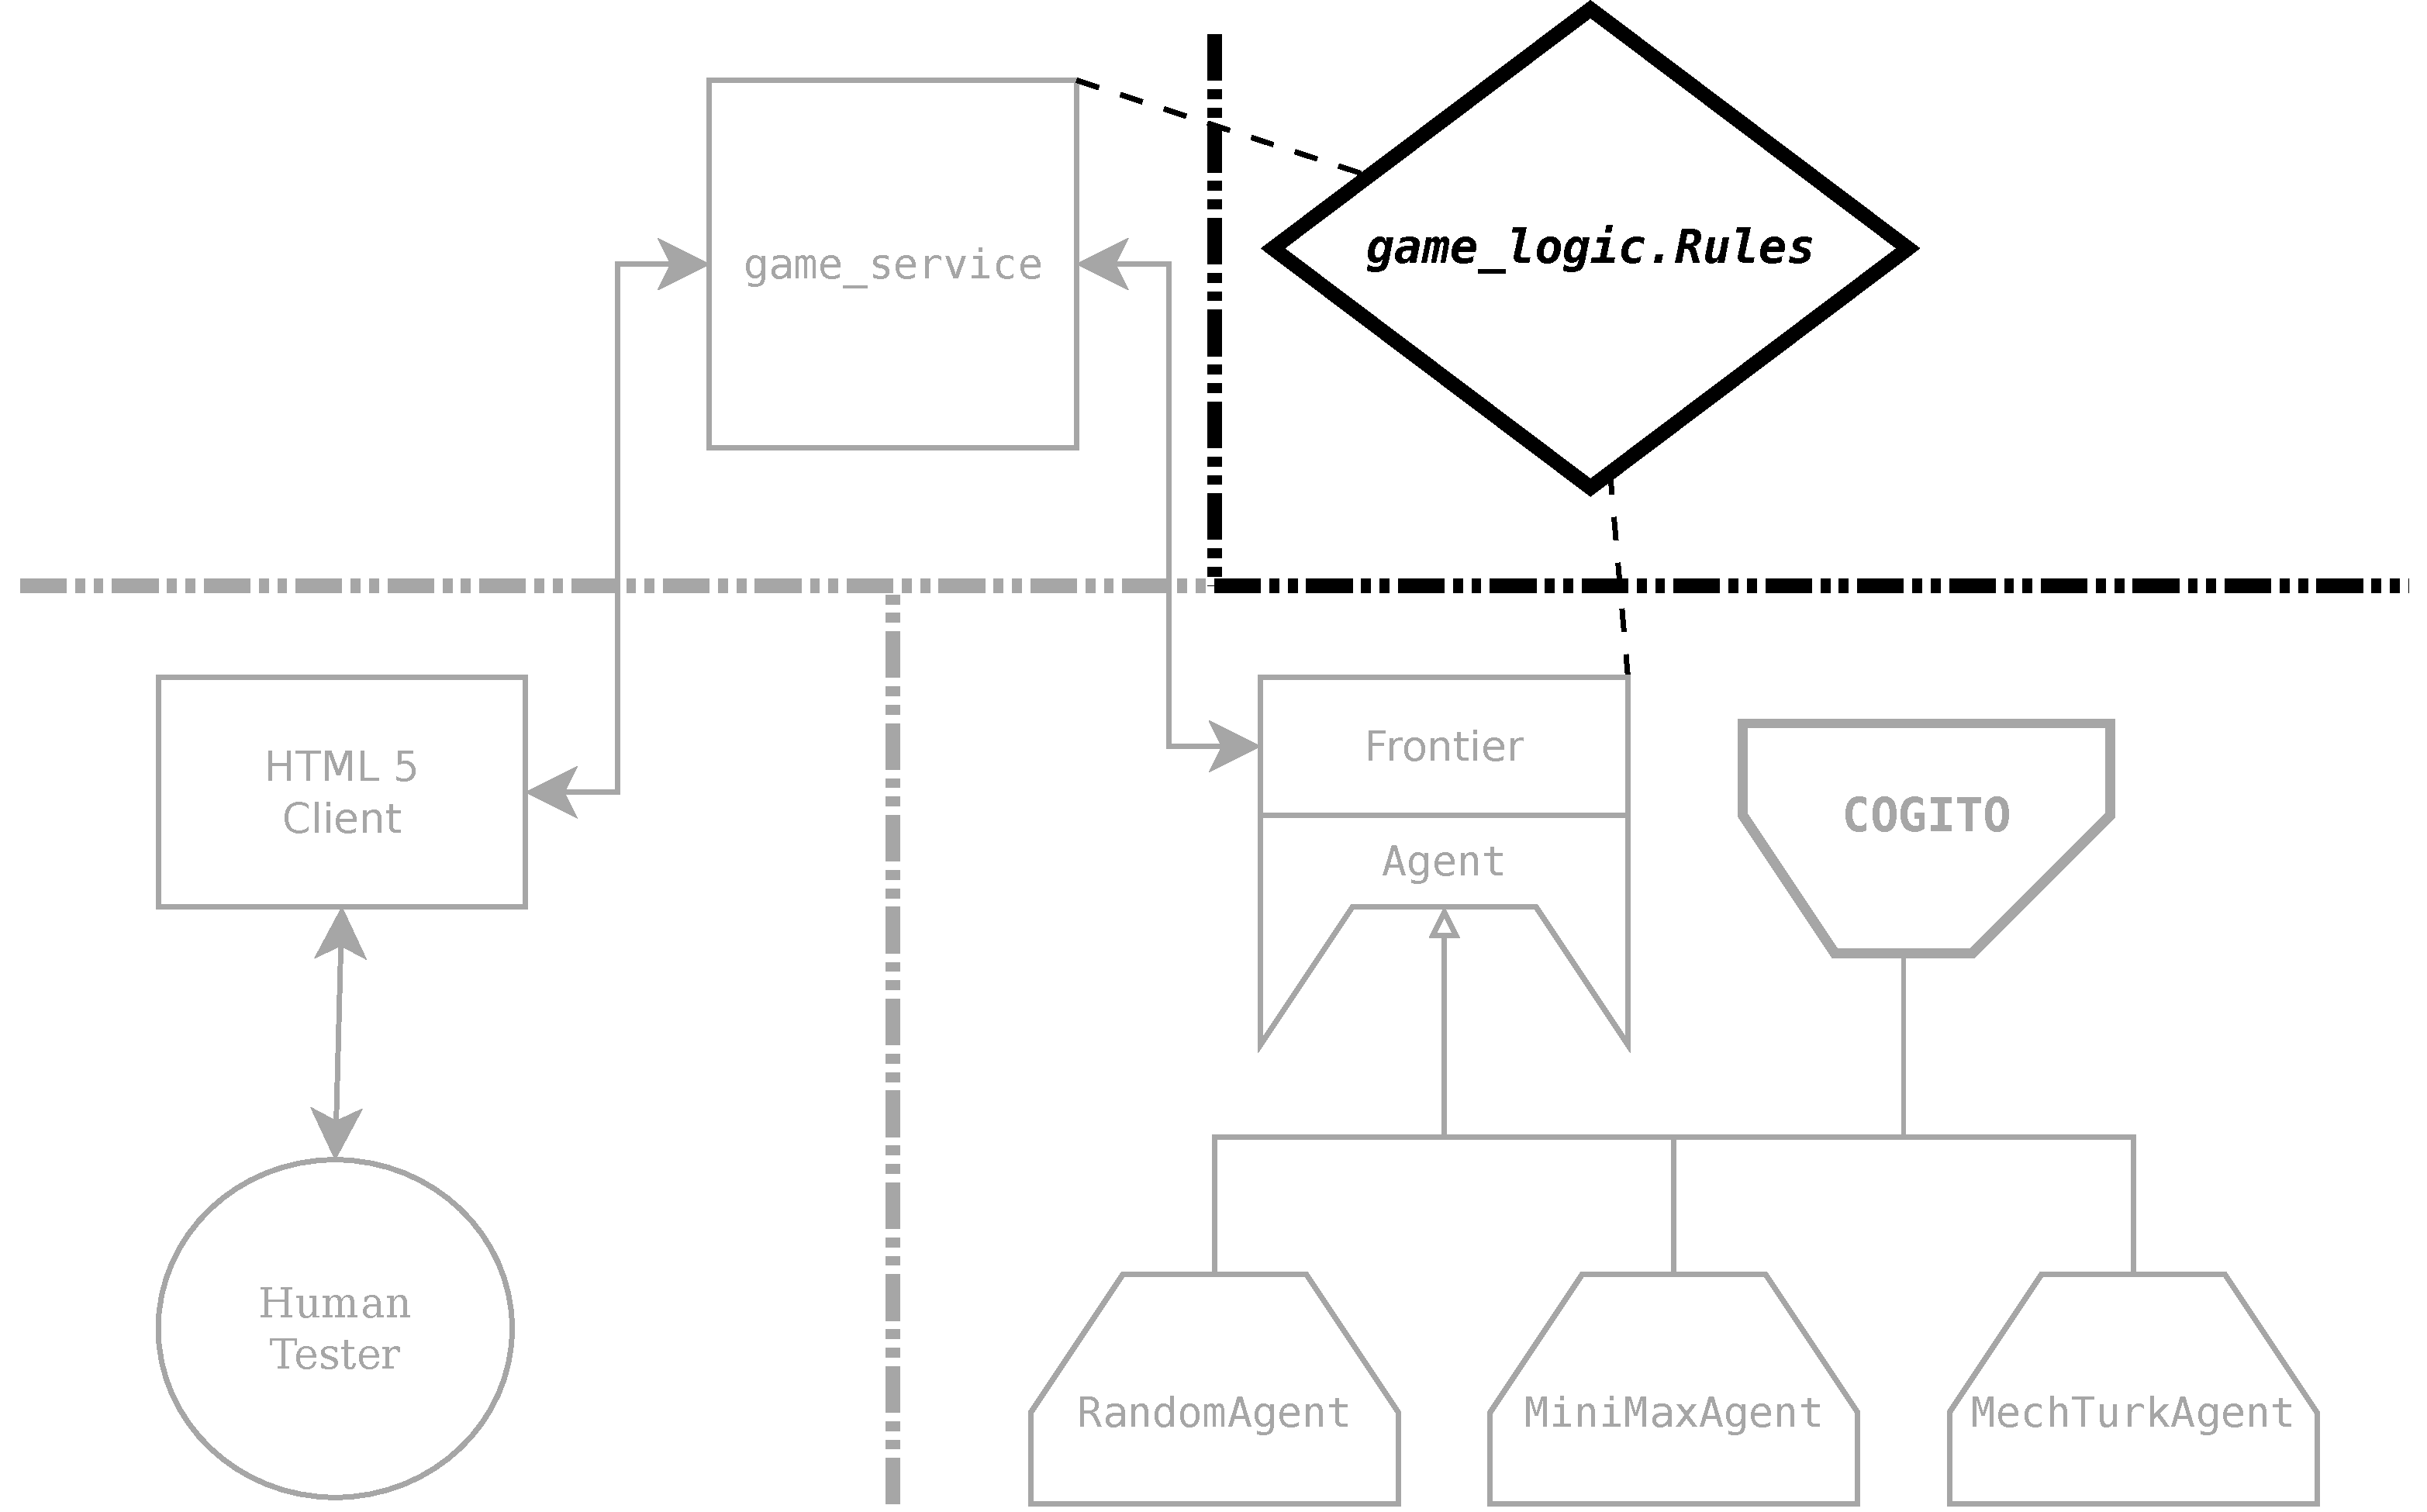
\includegraphics[width=0.8\textwidth]{img/william/archi_lib}\\
\end{center}
\end{frame}
%----------------------------------------
% GAME_LOGIC -- IN DEPTH
%----------------------------------------
%\begin{frame}{Environnement}{Bibliothèque \texttt{game\_logic}}
%\begin{center}
%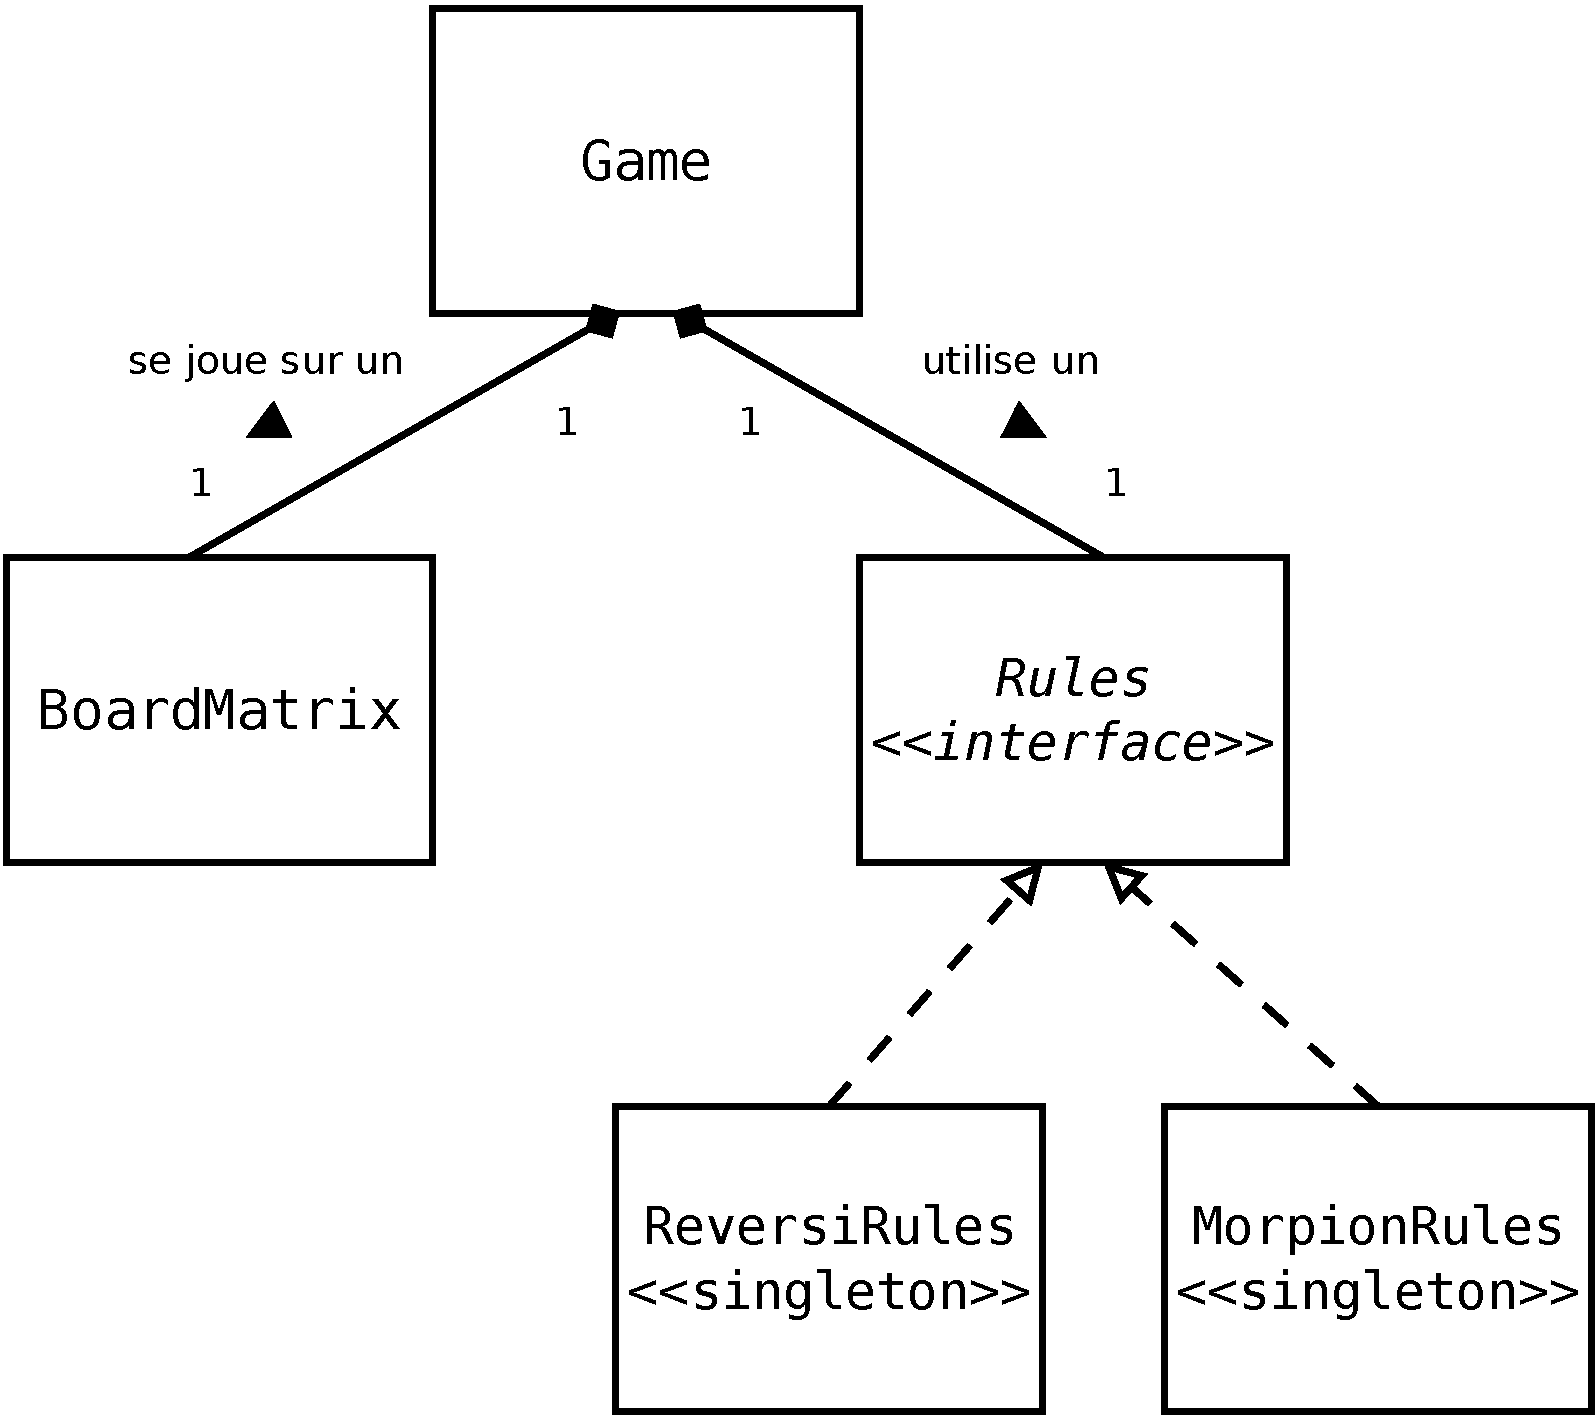
\includegraphics[height=0.5\textwidth]{img/william/game_logic}\\
%\end{center}
%\end{frame}
%----------------------------------------
% SERVEUR -- IN DEPTH
%----------------------------------------
%\begin{frame}{Environnement}{Serveur \texttt{game\_service}}
%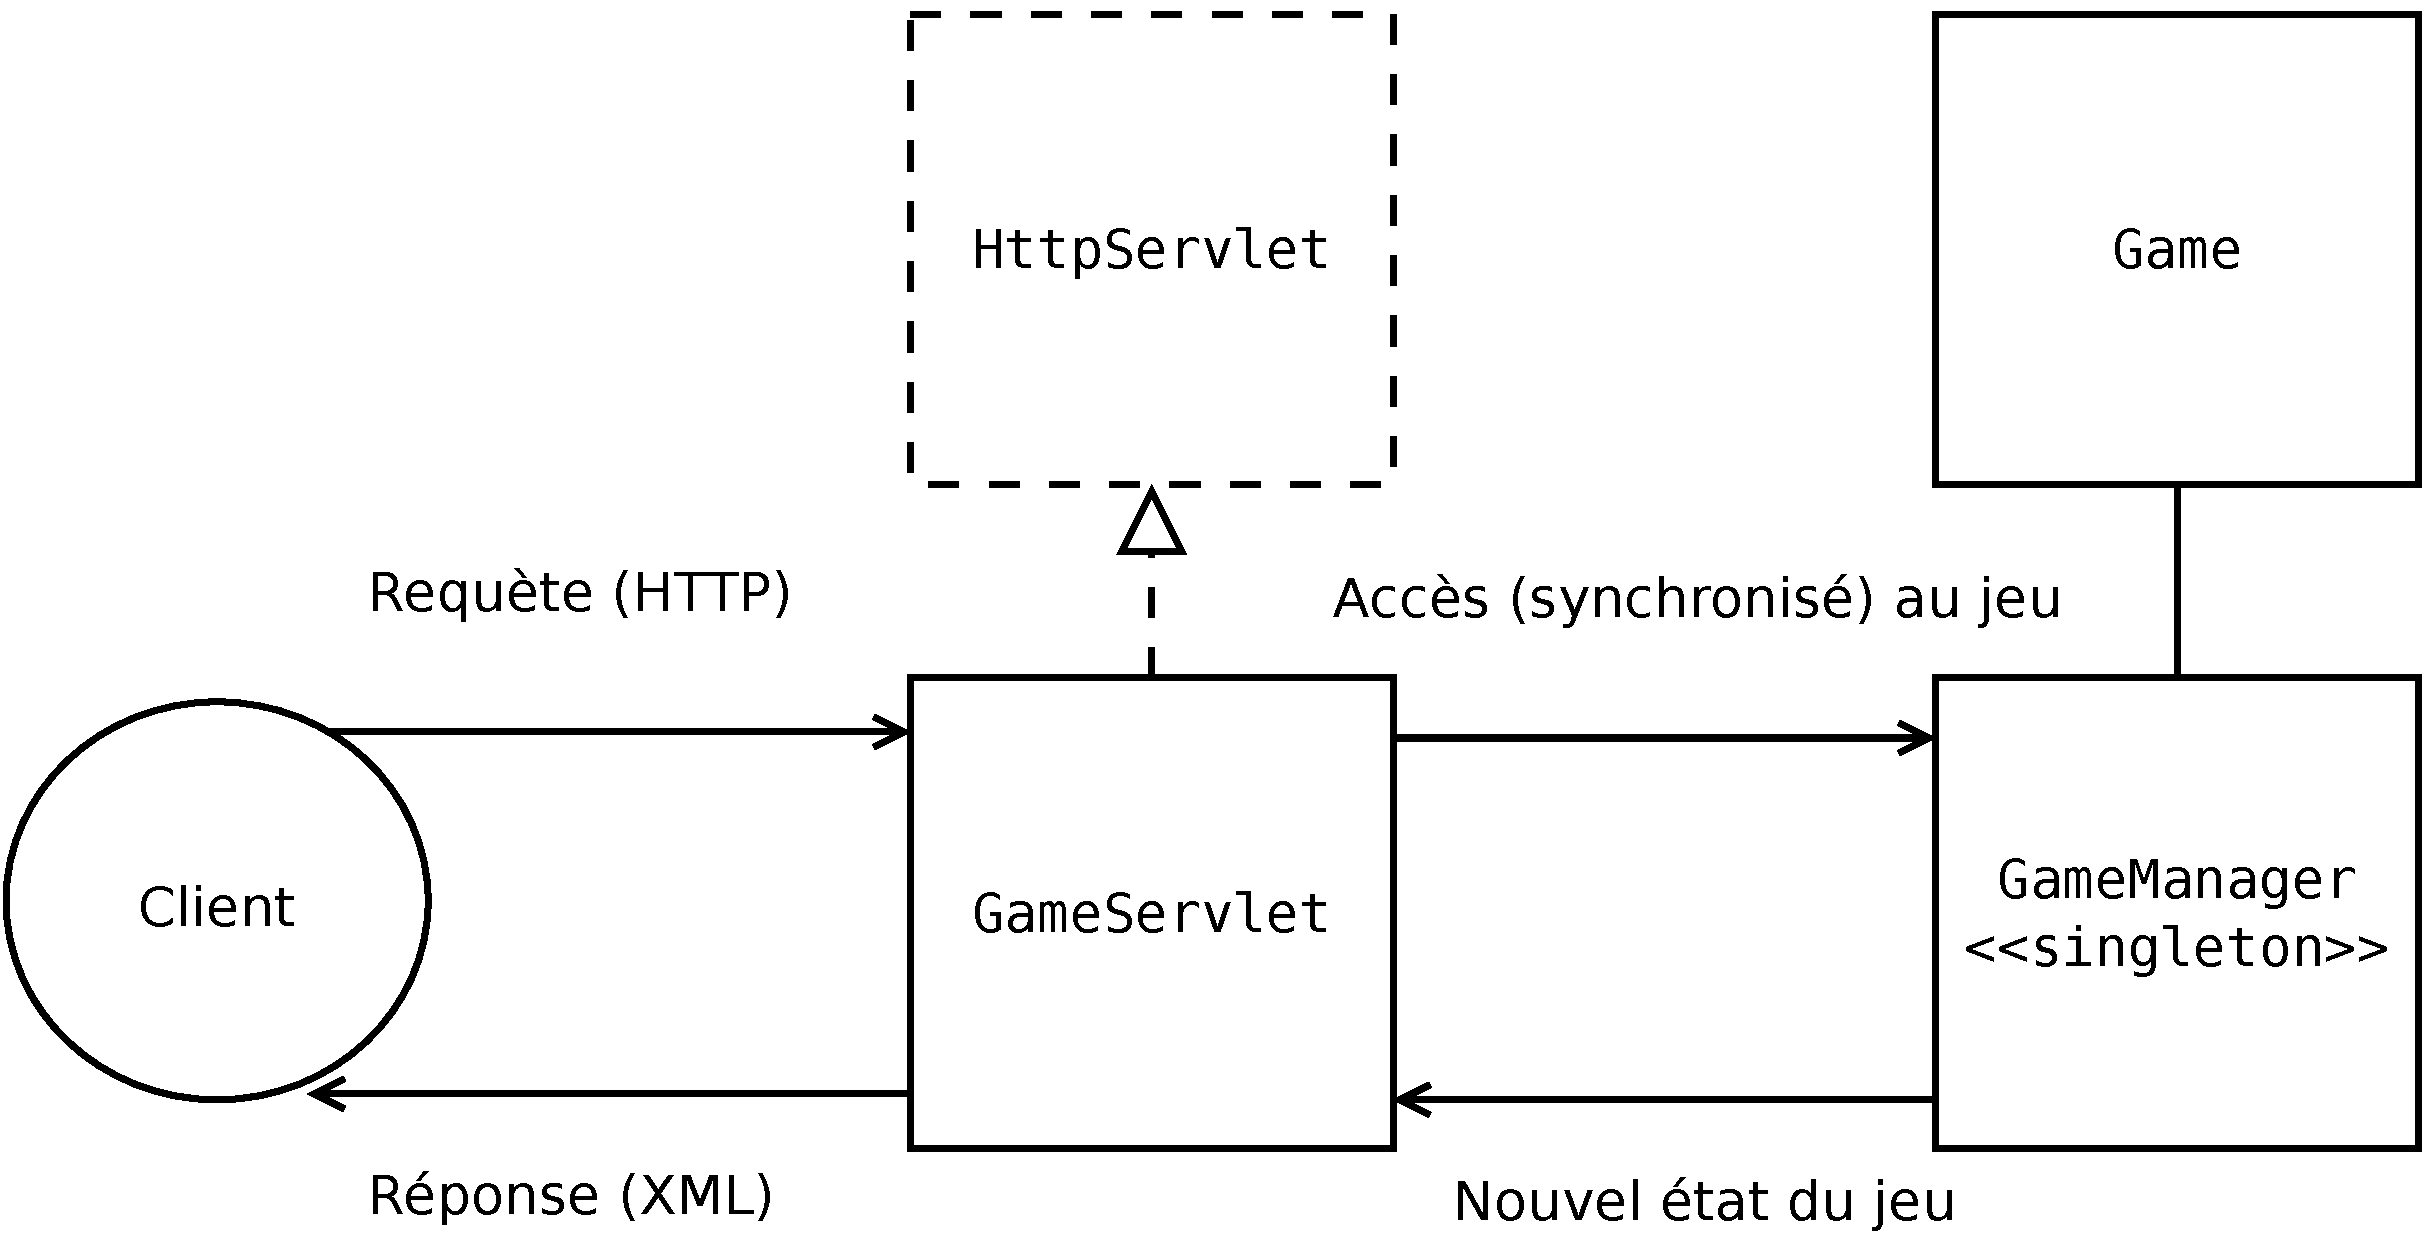
\includegraphics[width=\textwidth]{img/william/game_service}\\
%\end{frame}
%----------------------------------------
% PASSONS À COGITO
%----------------------------------------
\begin{frame}{Environnement}{Agents}
\begin{center}
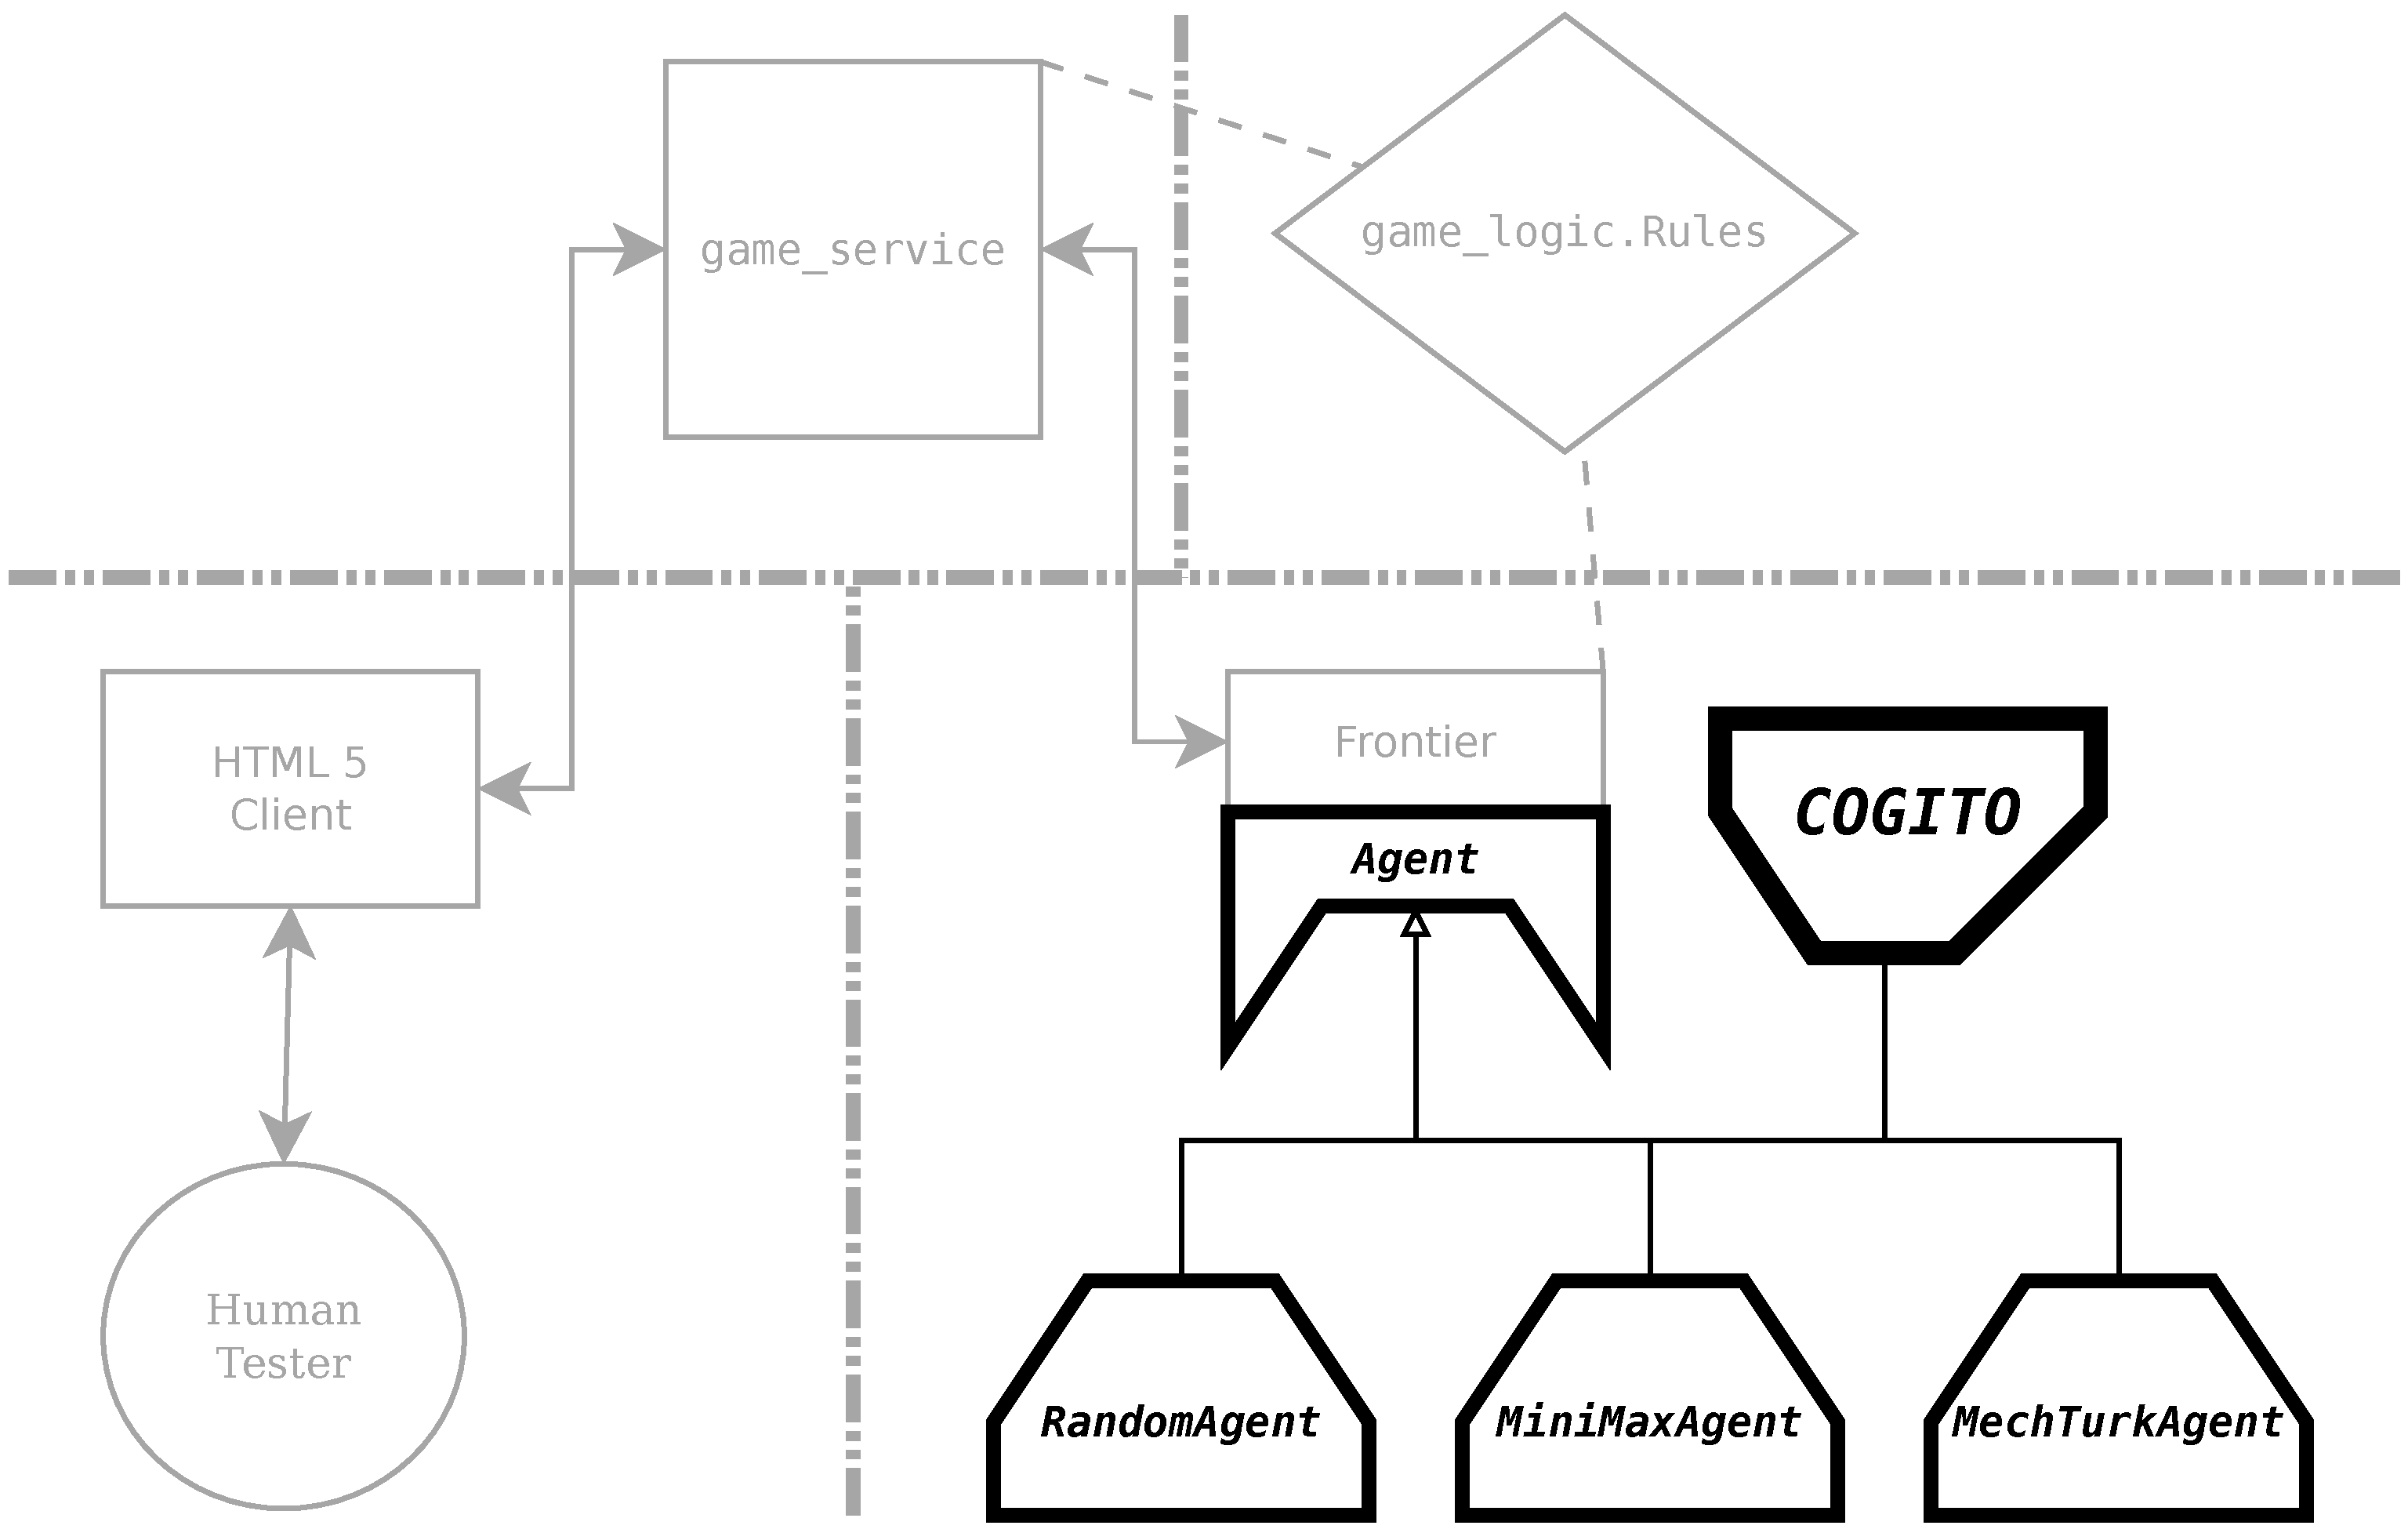
\includegraphics[width=0.8\textwidth]{img/william/archi_agents}\\
\end{center}
\end{frame}

\subsection{Généralités}
\begin{frame}{Généralités}{Séquence d'un coup}
modified simplified general diagram
\end{frame}



\subsection{Analyseur conceptuel}
\begin{frame}{Analyseur conceptuel}{Généralités}
\begin{itemize}
  \item Représente les connaissances tirées de l'environnement
  \item Analyse des connaissances afin d'en extraire de nouvelles
\end{itemize}
\end{frame}

\begin{frame}{Analyseur conceptuel}{Analyse détaillée}
\begin{itemize}
  \item Représentation des connaissances : \textbf{vocabulaire}
  \begin{itemize}
    \item Formules logiques (logique du premier ordre)
  \end{itemize}
  \pause
  \item Analyse des connaissances : \textbf{mécanisme}
  \begin{itemize}
    \item Recherche d'homomorphismes
  \end{itemize}
\end{itemize}
\end{frame}

\begin{frame}{Analyseur conceptuel}{Implémentation : rôles du module}
\begin{itemize}
  \item \textbf{Convertisseur :}
  \begin{itemize}
    \item Rend les données de l'environnement \enquote{lisibles} par l'IA
  \end{itemize}
  \item \textbf{Moteur d'inférence :}
  \begin{itemize}
    \item Applique les règles générées par l'IA afin d'en
    extraire de nouvelles informations
  \end{itemize}
\end{itemize}
\end{frame}

\begin{frame}{Analyseur conceptuel}{Implémentation : Classes principales}
\begin{itemize}
  \item \textbf {Choices (environnement)} : représente un plateau
  courant et l'ensemble des plateaux résultants des coups possibles
  \pause
  \item \textbf {BoardMatrix (environnement)} : représente un plateau sous forme
  matricielle
  \pause
  \item \textbf {Choices\_FOL (IA)} : version logique du premier ordre de
  Choices (même structure, attributs décrits par des formules logiques)
  \pause
  \item \textbf {CompleteBoardState (IA)} : version logique du premier ordre de
  BoardMatrix (classe qui décrit la configuration
  d'un plateau complet comme une liste de faits logiques)
  \pause
  \item \textbf {RelevantPartialBoardState (IA)} : classe qui décrit la
  configuration d'une sous-partie pertinente d'un plateau comme une règle
  logique 
\end{itemize}
\end{frame}


\begin{frame}{Analyseur conceptuel}{Implémentation détaillée}
\begin{itemize}
  \item \textbf {Convertisseur} :
  \begin{itemize}
    \item Entrée (de l'environnement): instance de \texttt{Choices}
    \pause
    \item Génération de faits logiques représentant la configuration d'un
    plateau en forme matricielle (\texttt{BoardMatrix})
    \pause
    \item Base de faits correspondante stockée dans une instance de
    \texttt{CompleteBoardState}
    \pause
    \item Sortie: instance de
    \texttt{Choices\_FOL}
  \end{itemize}
\end{itemize}
\end{frame}

\begin{frame}{Analyseur conceptuel}{Implémentation détaillée}
\begin{itemize}
\item \textbf {Moteur d'inférence} :
\begin{itemize}
  \item Entrée (de la mémoire) : liste de \texttt{RelevantPartialBoardState},
  règles du type : 
  \pause
  \emph{$isCorner(x) \wedge isMine(x) \Longrightarrow \_rpbs034(x)$}
  \pause
  \item Saturation de la base de faits des \texttt{CompleteBoardState} en
  appliquant l'ensemble de ces règles
  \pause
  \item Reconnaissance de formes : recherche d'homomorphisme entre l'atome de
  conclusion de la règle (\texttt{RelevantPartialBoardState}) et la base de
  faits de chaque plateau
  \pause
  \item Ajout de la liste de \texttt{RelevantPartialBoardState} présents dans
  chaque \texttt{CompleteBoardState} du paquet \texttt{Choices\_FOL}
  \pause
  \item Appel à la méthode \texttt{stimulate} du module de raisonnement
  \item Sortie (passée à la mémoire) : instance de \texttt{Choices\_FOL}
\end{itemize}
\end{itemize}
\end{frame}


\subsection{Raisonneur}
\begin{frame}{Raisonneur}{Moteur de choix}
Proba / Bayes
\end{frame}

\begin{frame}{Raisonneur}{Moteur d'introspection}
Comparaison de représentation mémorisé de l'environnement, afin d'en extraire des sous partie commune (RPBS)
\end{frame}

\subsection{Mémoire}
\subsubsection{Interface Mémoire}

Le module de mémoire a été conçu de manière générique à l'aide d'interfaces java. Pour cela elle se décompose en trois parties :

\begin{itemize}
\item l'interface principale de la mémoire, qui déclare les méthodes appelées par les autres modules (Analyse et Raisonnement), et qui est implémentée en tant que mémoire à court terme (ActiveMemory),

\item l'interface de la mémoire épisodique et l'interface de la mémoire sémantique, qui déclarent les méthodes appelées par le module Mémoire.
\end{itemize}

\begin{figure}[H]
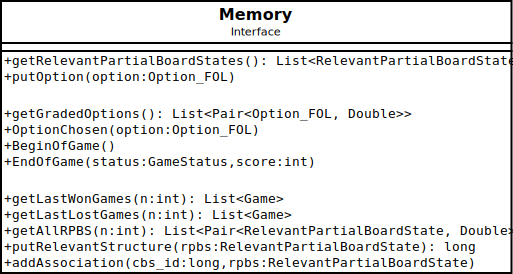
\includegraphics[width=\textwidth]{files/memoire/interface}
\caption{Interface mémoire}
\end{figure}

La mémoire doit également assurer la persistance des données, qui se fait via un module de persistance. Celui-ci est utilisé par une implémentation spécifique des interfaces décrites ci-avant.

\subsubsection{Le \gls{SGBD} Neo4j}

La persistance des données est assurée par un SGBD né de la mouvance \gls{NoSQL} : Neo4j. Il permet la gestion d'une base de données orientée graphe. Nous avons fait le choix d'utiliser un tel système pour plusieurs raisons :

\begin{itemize}
\item nous avions la volonté de découvrir une solution \gls{NoSQL}, que nous n'avons pas eu l'occasion d'étudier lors de notre formation,

\item Neo4j est disponible en plusieurs versions, notamment en version serveur, version webservice REST et version java embarquée. La mémoire n'étant pas accédée de manière concurrente ainsi que pour des soucis de légèreté, c'est la version embarquée (\emph{embedded java})qui a été utilisée,

\item ce type de \gls{SGBD} \gls{NoSQL} permet d'obtenir des temps d'accès plus rapides qu'avec des \gls{SGBD} relationnels traditionnels,

\item la vision graphe de la base de données est adaptée à la conception de notre mémoire\footnote{Notons tout de même qu'il aurait était été possible de stocker les données sous forme de tables},

\item cette solution conserve les propriétés \gls{ACID} des transactions des \gls{SGBD} relationnels traditionnels,

\item la documentation complète et la communauté active permettent de s'initier très rapidement à cette nouvelle technologie,

\item Neo4j est une solution libre distribuée sous licence \gls{GPLv3}.
\end{itemize}

Neo4j étant un \gls{SGBD} \gls{NoSQL} orienté graphe, la base de donnée est représentée sous la forme d'un graphe orienté, composé d'un nœud \og root \fg{}. Chaque nœud et chaque arc peut posséder des attributs. Cependant, il n'est possible de définir que des types d'arc, pour les nœuds on utilise donc une astuce qui consiste en la création d'un \og master\_node \fg{} comme le montre le schéma suivant : 

\begin{figure}[H]
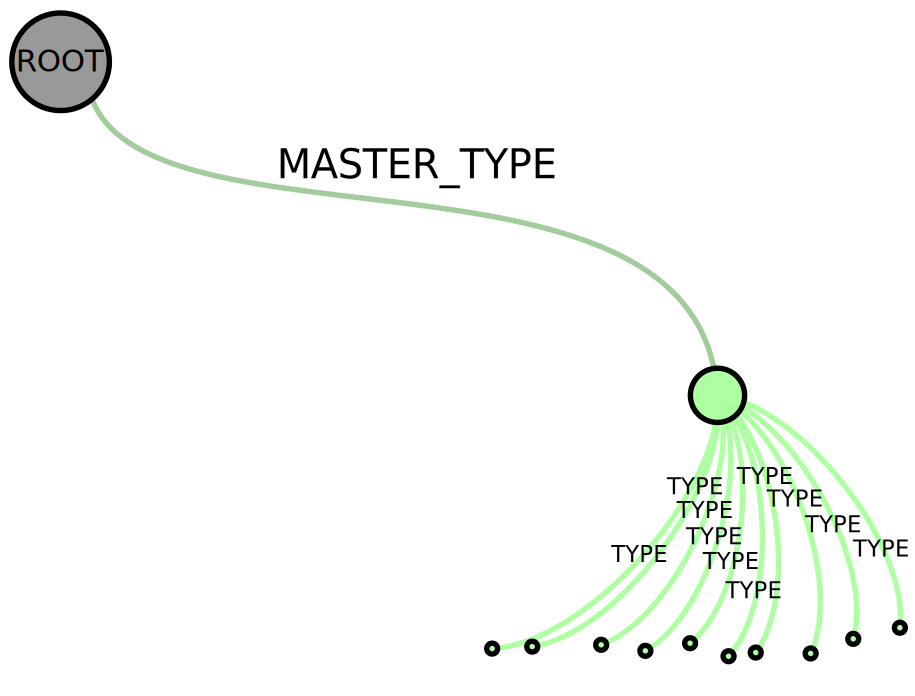
\includegraphics[width=\textwidth]{files/neo4j/example_node_type}
\caption{Exemple de typage des noeuds avec Neo4j.}
\label{example_node_type}
\end{figure}

\subsubsection{Éléments en mémoire}

Le module de persistance permet le stockage de la mémoire épisodique et sémantique, les deux étant liées par les relations entre les \emph{MOVE} et les \emph{CBS}. Nous avons donc besoin des types suivants : 

\textbf{Types de noeud :}
\begin{itemize}
	\item \texttt{GAME} : une partie en mémoire épisodique, 
	\item \texttt{MOVE} : un coup joué en mémoire épisodique,
	\item \texttt{CBS} : un \texttt{CBS} en mémoire sémantique,
	\item \texttt{RPBS} : un \texttt{RPBS} en mémoire sémantique.
\end{itemize}


\textbf{Types de liens :}
\begin{itemize}
	\item Relations maitres
		\begin{itemize}
			\item \texttt{MASTER\_ATTR},
			\item \texttt{MASTER\_OBJ},
			\item \texttt{MASTER\_GAME},
			\item \texttt{MASTER\_MOVE}.
		\end{itemize}
	\item Relations de type
		\begin{itemize}
			\item \texttt{ATTRIBUTE},
			\item \texttt{OBJECT},
			\item \texttt{MOVE},
			\item \texttt{GAME},
			\item \texttt{LAST\_GAME} (relation \texttt{GAME} spéciale, signifiant que cette partie est la dernière jouée).
		\end{itemize}
	\item Relations en mémoire épisodique
		\begin{itemize}
			\item \texttt{PREV\_GAME} : permet à partir d'une partie d'accéder à la précédente,
			\item \texttt{LAST\_MOVE} : permet à partir d'une partie d'accéder au dernier coup joué,
			\item \texttt{PREV\_MOVE} : permet à partir d'un coup d'accéder au précédent,
			\item \texttt{STATE\_BOARD} : permet de lier un coup à l'état de plateau correspondant.
		\end{itemize}
	\item Relations en mémoire sémantique
		\begin{itemize}
			\item \texttt{RELATED} : décrit la présence d'un \texttt{RPBS} dans un \texttt{CBS}.
		\end{itemize}
	\end{itemize}
	
\subsubsection{Mémoire sémantique}
Comme vu dans la partie~\ref{conception_memoire_semantique} (page \pageref{conception_memoire_semantique}, la mémoire sémantique stocke une matrice de booléens ayant comme attributs (colonnes) des \texttt{RPBS}, et comme objets (lignes) des \texttt{CBS}.

On peut voir sur la figure~\ref{lattice_graph} les deux \og master\_node \fg{} permettant de déclarer des nœuds d'attributs et d'objets. Ces noeuds sont en liés via des relations de type \emph{RELATED}.

\begin{figure}[H]
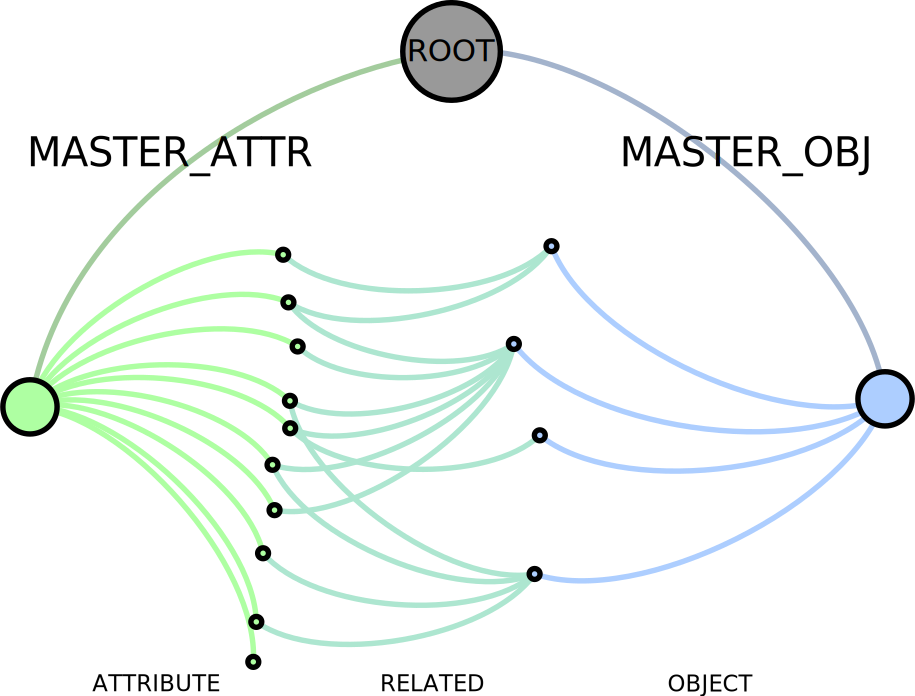
\includegraphics[width=\textwidth]{files/neo4j/lattice_graph}
\caption{Représentation de la mémoire sémantique dans Neo4j.}
\label{lattice_graph}
\end{figure}

\subsubsection{Mémoire épisodique}

La représentation sous forme de graphe se prête parfaitement à la mémorisation des parties et des coups sous la forme d'une double liste chaînée. La figure~\ref{episodic_graph} représente la mémoire épisodique telle qu'elle est stockée dans Neo4j.

On visualise parfaitement les trois \og master\_node \fg{} permettant de typer les \texttt{GAME}, \texttt{MOVE} et \texttt{ATTRIBUTES}. Le parcours des parties se fait via la relation \texttt{PREV\_GAME} et celui des coups via la relation \texttt{PREV\_MOVE}.

On remarque également que les relations \texttt{BOARD\_STATE} permettent de faire la liaison entre la mémoire sémantique et la mémoire épisodique.

\begin{figure}[H]
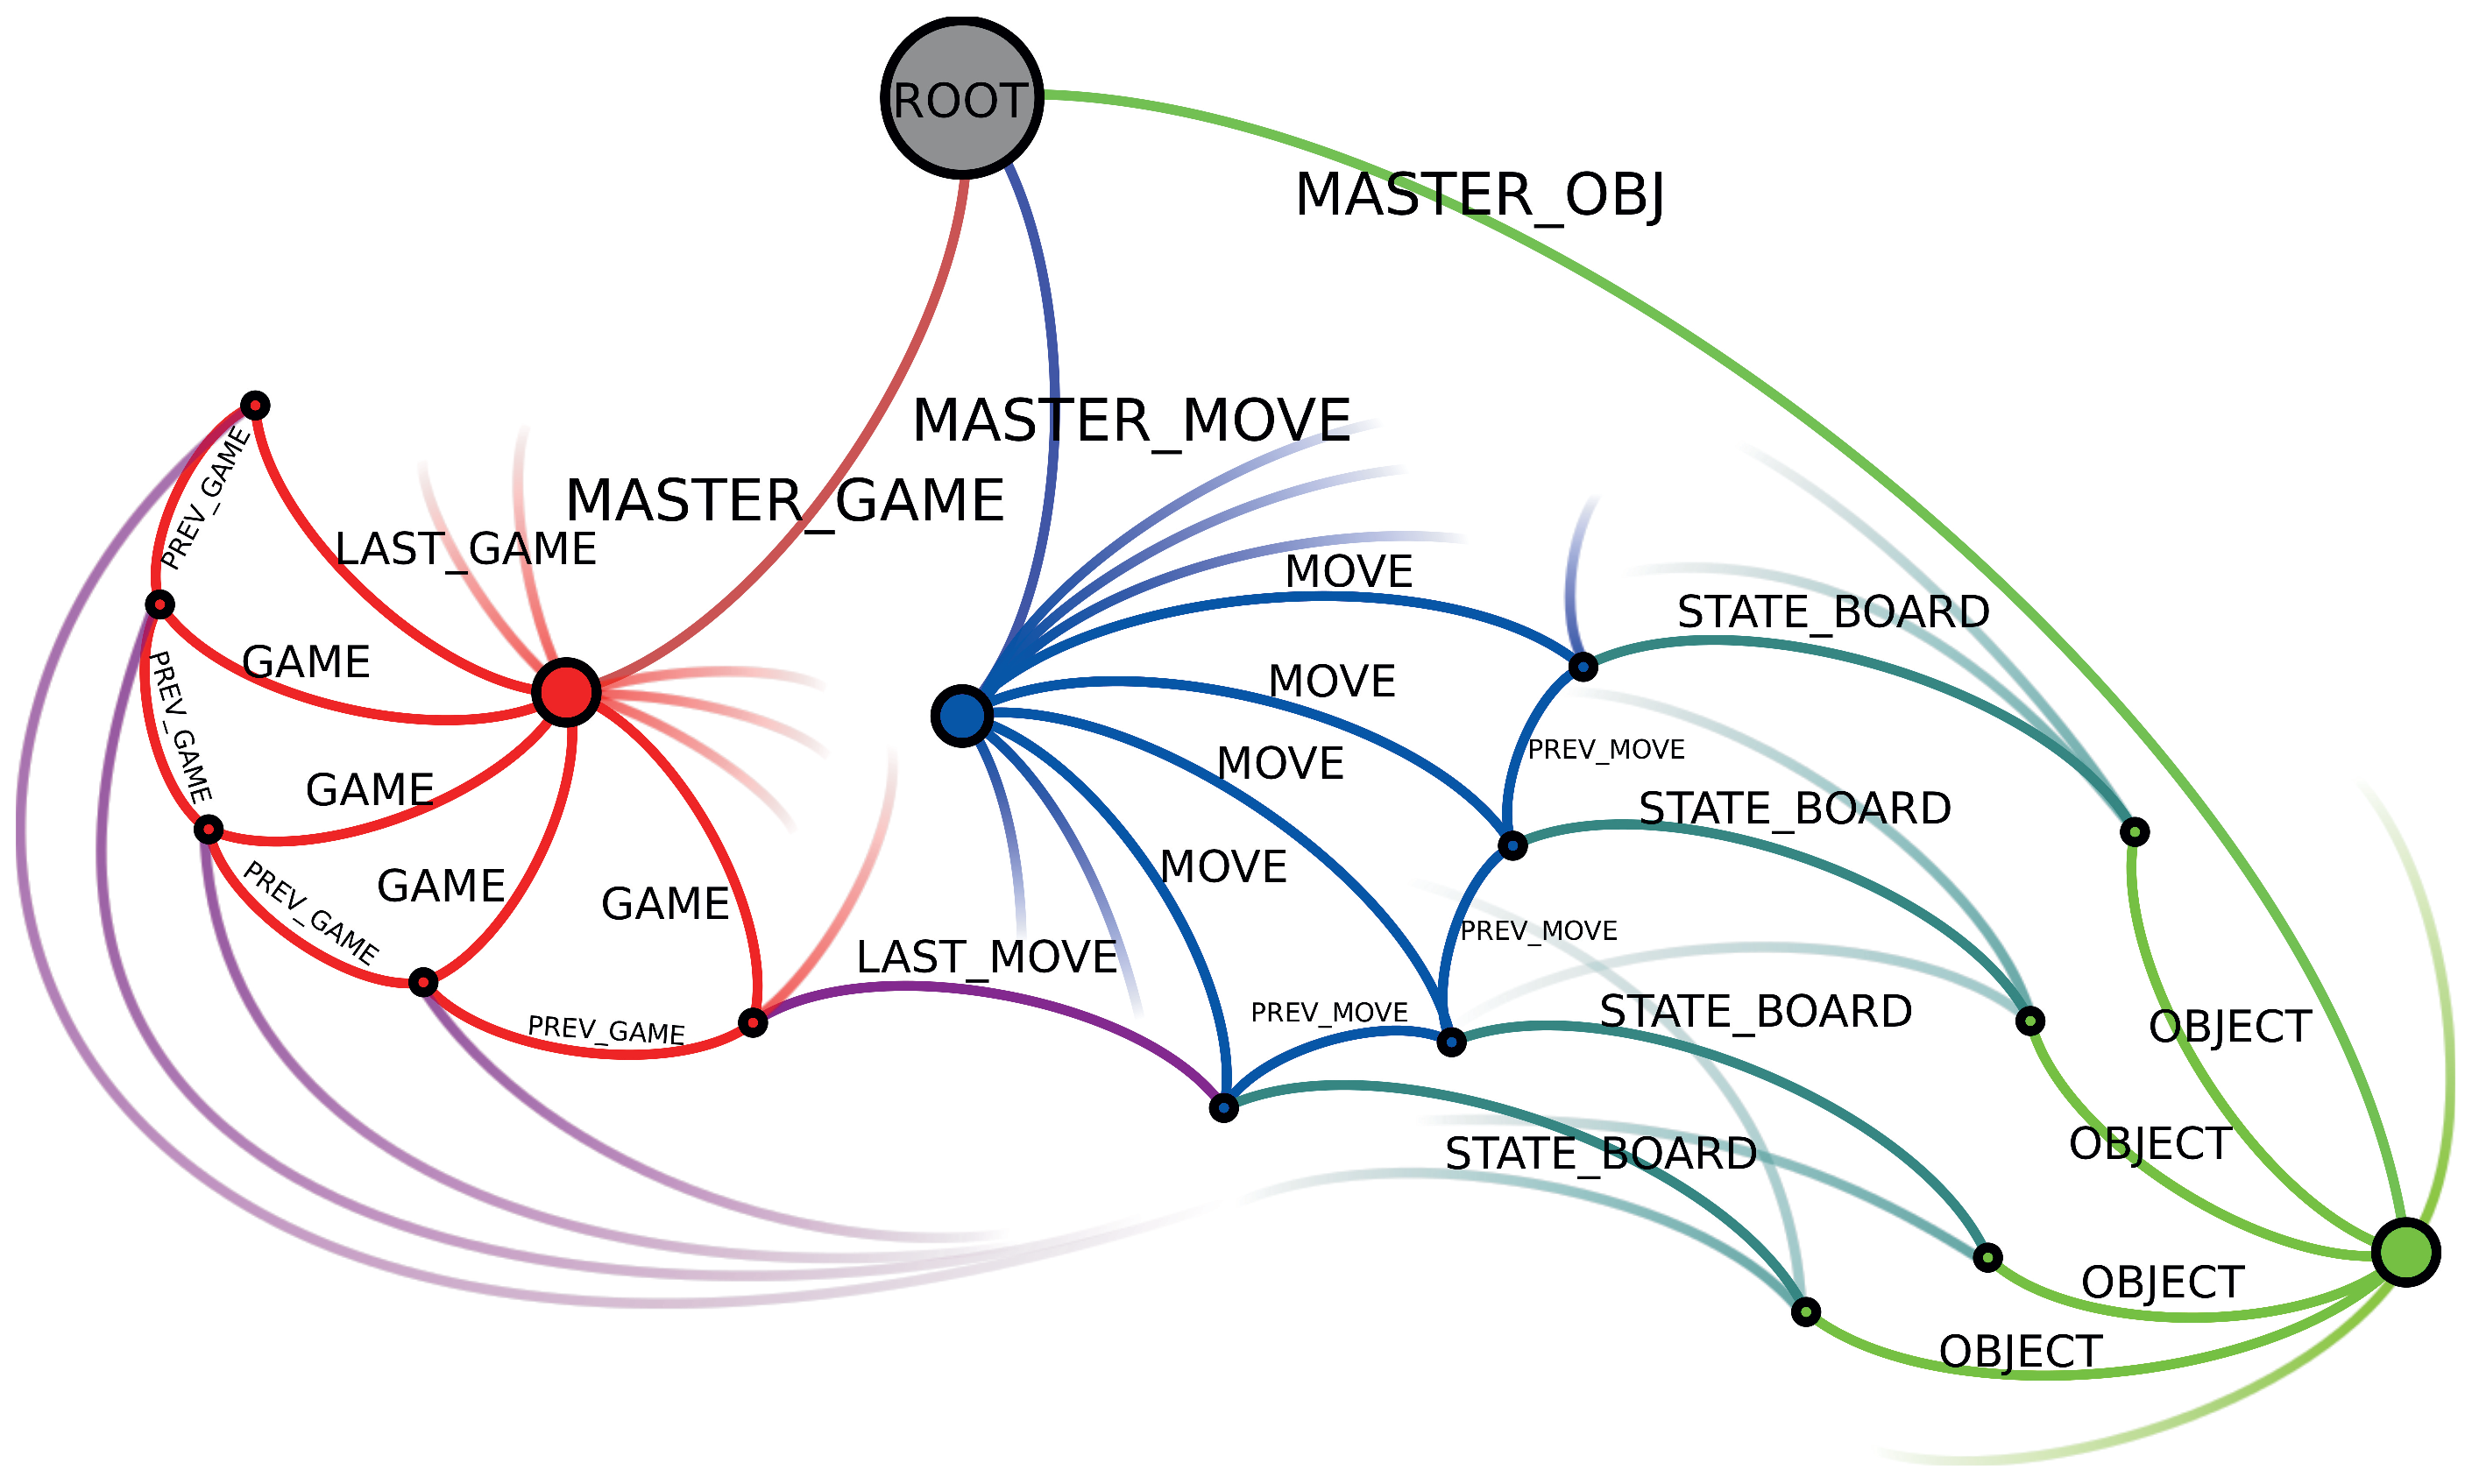
\includegraphics[width=\textwidth]{files/neo4j/episodic_graph}
\caption{Représentation de la mémoire épisodique dans Neo4j.}
\label{episodic_graph}
\end{figure}

\subsubsection{Vision globale de la mémoire}

La figure~\ref{full_graph} présente le stockage de la mémoire épisodique et de la mémoire sémantique dans Neo4j. Les relations de type \texttt{BOARD\_STATE} assure la liaison entre ces deux mémoires.
\begin{figure}[H]
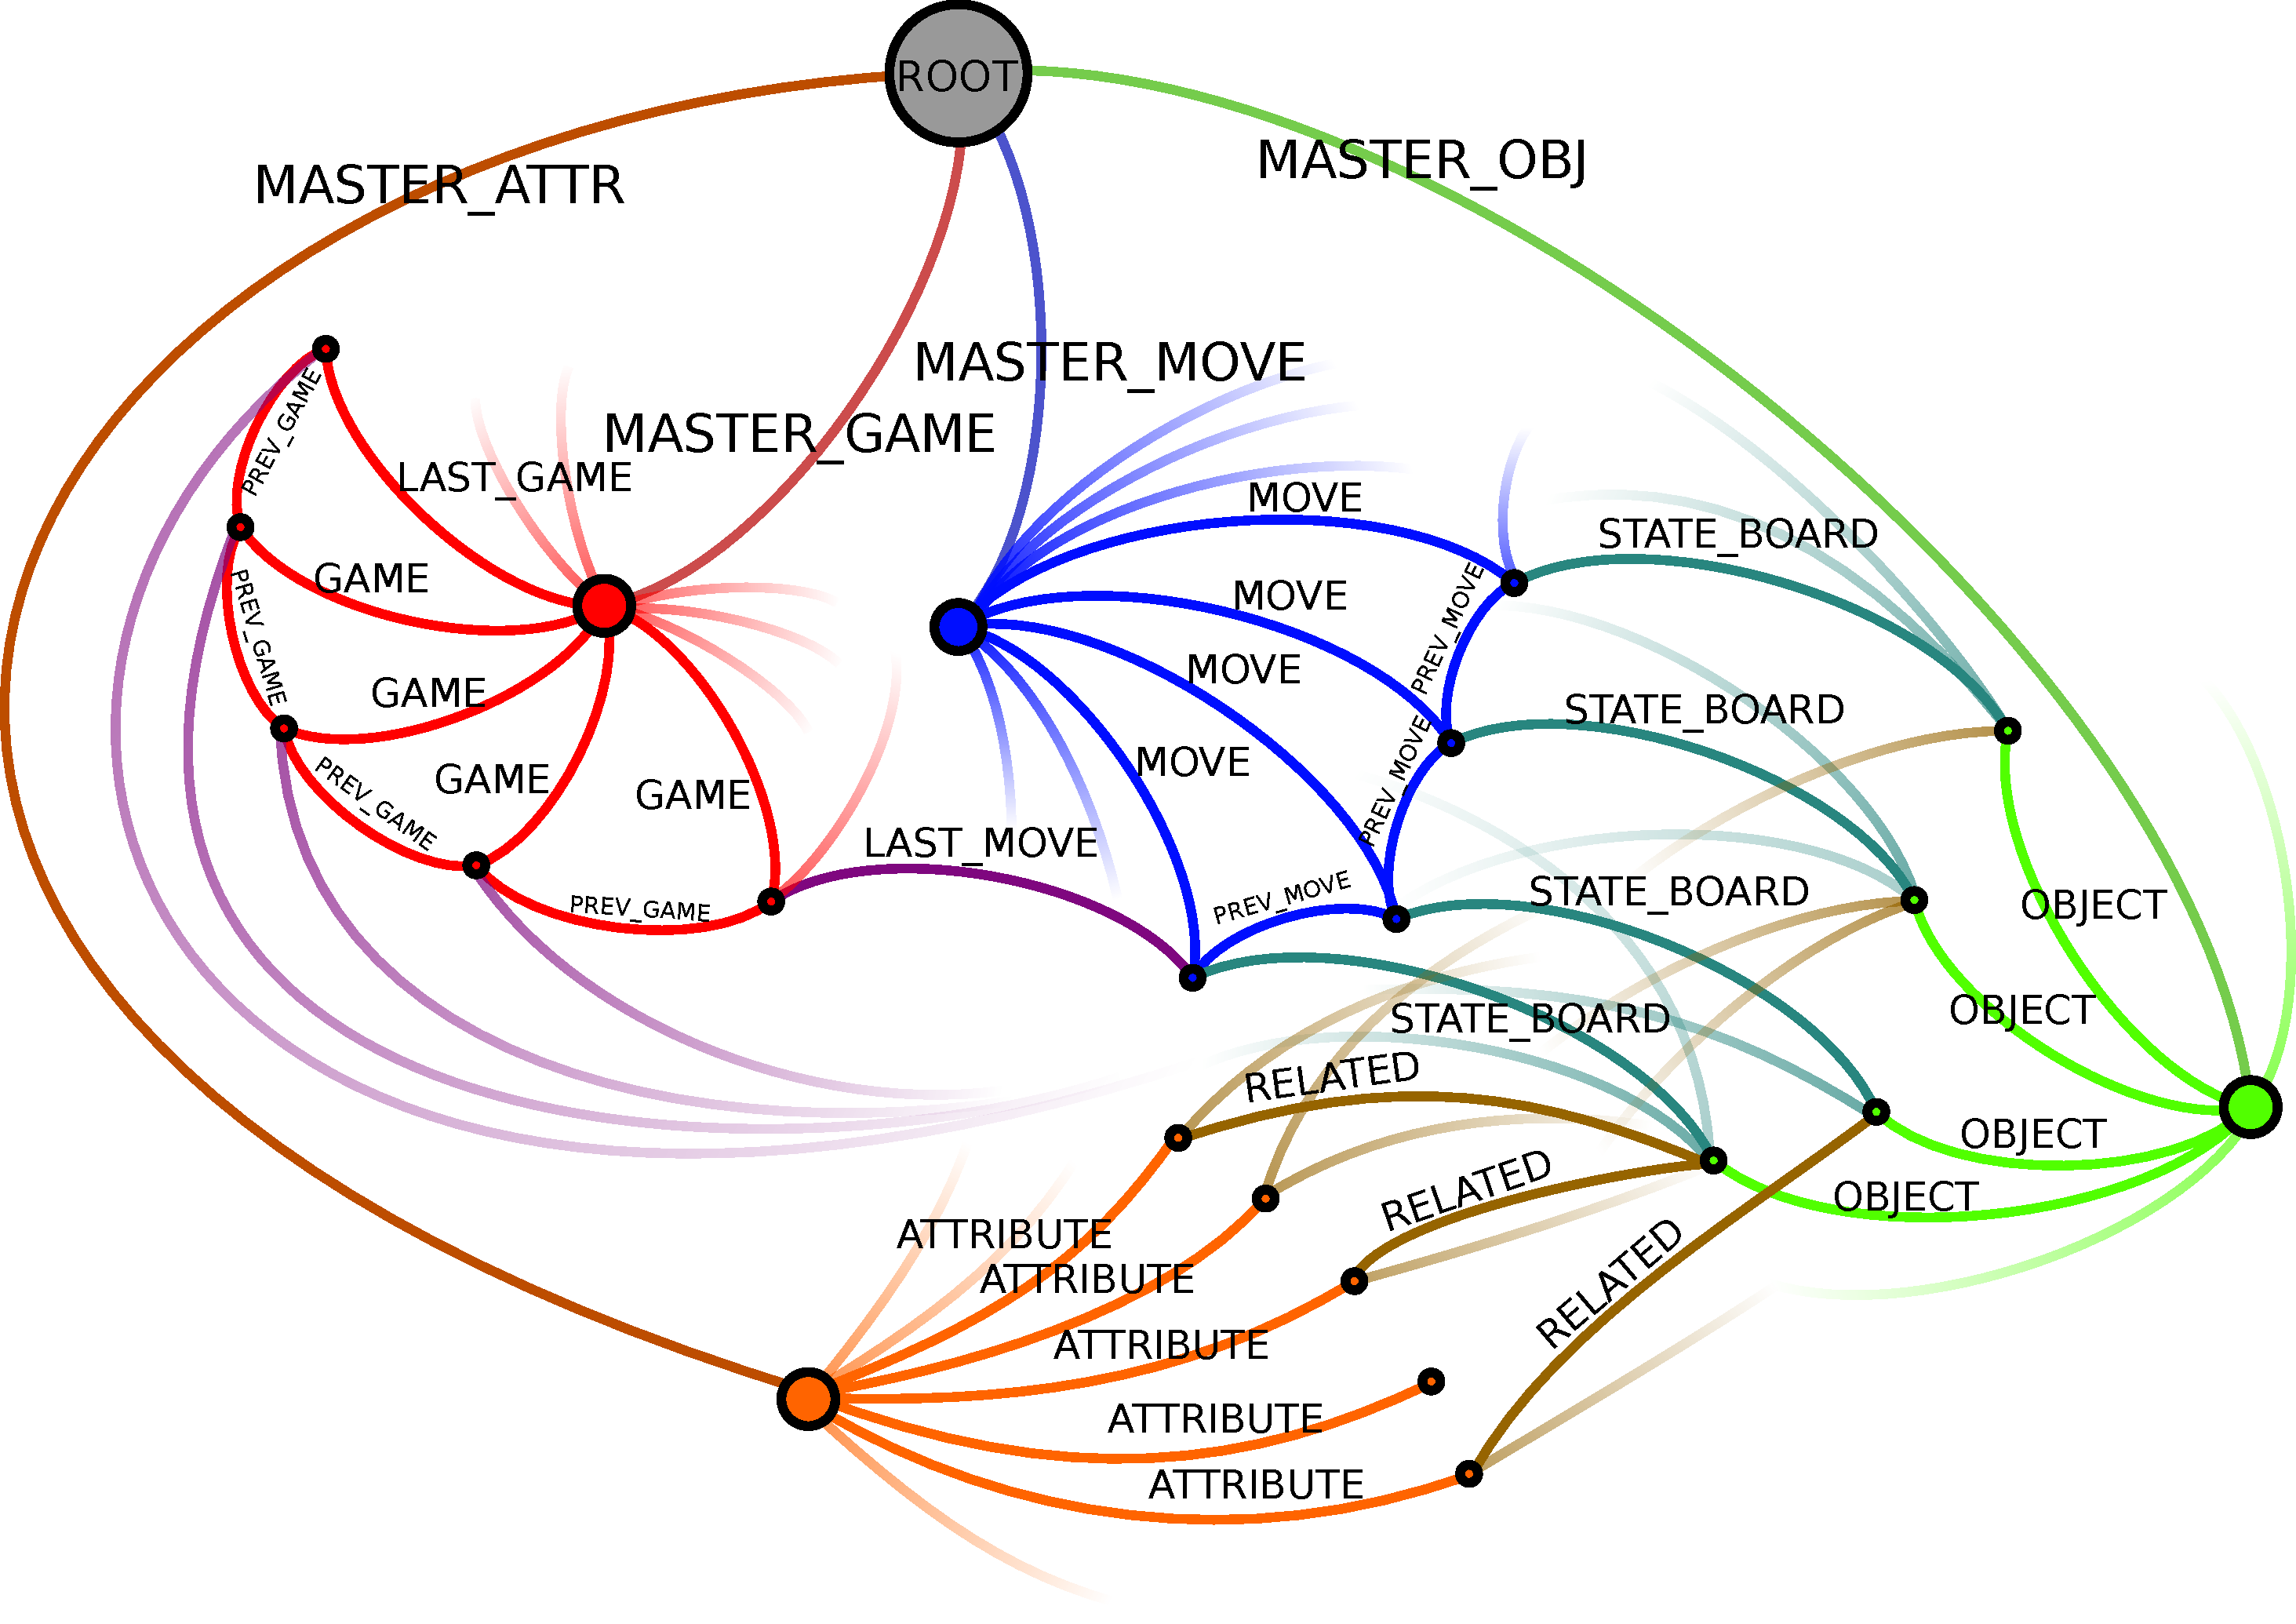
\includegraphics[width=\textwidth]{files/neo4j/full_graph}
\caption{Représentation complète de la mémoire stockée dans Neo4j.}
\label{full_graph}
\end{figure}

\subsection{Conclusion partielle}
\clearemptydoublepage
\chapter{Résultats \&  discussion}

\section{Résultats}



\section{Discussion}
\subsection{Un treillis en mémoire ?}
Comme nous l'avons vu dans la partie~\ref{conception_memoire_semantique} (page \pageref{conception_memoire_semantique}), la mémoire sémantique entrepose une matrice de booléens associant des formes remarquables à des plateaux. Ces associations correspondent typiquement à la définition d'un contexte, permettant la construction d'un treillis de concepts.

\subsubsection{Analyse de concepts formels}
FCA\footnote{Formal Concept Analysis (en Français \og Analyse de Concepts Formels \fg{}).} est l'étude de concepts définis de manière formelle, via un contexte. Cette section ne présente pas en détail FCA. Pour plus d'informations sur cette méthode d'analyse et les treillis de Galois nous vous recommandons la lecture des cours de Marianne Huchard et de Michel Liquière\footnote{Cours de Marianne Huchard, Professeur en informatique à l'université Montpellier 2 (Faculté des Sciences) et Directrice adjointe du LIRMM (Laboratoire d'Informatique, de Robotique et de Microélectronique de Montpellier) et de Michel Liquière, Maitre de Conférences dans la même université, disponibles à l'adresse suivante : \texttt{http://www.lirmm.fr/\textasciitilde huchard/Huchard/teaching.html}}.

\paragraph{Le contexte} Il s'agit d'un triplet $(G,M,I)$ avec $G$ et $M$ des ensembles et $I\subseteq G \times M$ des relations de $G$ dans $M$. Les éléments contenus dans $G$ sont appelés \emph{objets} et ceux de $M$ \emph{attributs}. $I$ est une relation entre une object de $G$ et un attribut de $M$, et qui se dit \og l'objet $g$ possède l'attribut $m$ \fg{}. (Source : Wikpiedia\footnote{L'article \og Analyse de concepts formels \fg{} de Wikipedia en Français à considérablement aidé à la rédaction de cette partie. Contenu sous licence CC-BY-SA.})

En application à \emph{COGITO} nous aurions :

\begin{tabular}{r c l}
$G$ & $ = $ & ensemble des plateaux (objets),\\
$M$ & $ = $ & ensemble des formes remarquables (attributs),\\
$I$ & $ = $ & ensemble des relations plateaux / formes remarquables\\
& & définies dans la matrice actuelle.\\
\end{tabular}

Construire des concepts à partir du contexte formel permettrait de raisonner à un niveau d'abstraction supplémentaire. Actuellement \emph{COGITO} travail sur des formes remarquables, après la construction d'un treillis de Galois, il pourrait raisonner sur des ensembles de formes remarquables.




\section{Outils de travail}
\begin{frame}{Outils de travail}{GIT - Un gestionnaire de version décentralisé}
\begin{tabular}{l r}
\begin{minipage}{0.5\textwidth}

\includegraphics[width=0.7\textwidth]{img/outils/git}\\
\begin{itemize}
\item Logiciel libre (GNUv2)
\item Simple d'utilisation
\item Hébergement via GitHub
\texttt{\small https://github.com/marminthibaut/artificial\_consciousness/}
\end{itemize}
\end{minipage} & \begin{minipage}{0.5\textwidth}\begin{center}

\includegraphics[width=0.2\textwidth]{img/outils/github_logo} \\

\includegraphics[width=0.5\textwidth]{img/outils/github_octocat}
\end{center}
\end{minipage}
\end{tabular}
\end{frame}

\begin{frame}{Rédaction collaborative}{Etherpad}

\end{frame}

\begin{frame}{Outils de travail}{Plateforme / Javadoc}

\end{frame}

\section{Conclusion \& Perspectives}
\subsection{Conclusion}
\clearemptydoublepage
\chapter{Résultats \&  discussion}

\section{Résultats}



\section{Discussion}
\subsection{Un treillis en mémoire ?}
Comme nous l'avons vu dans la partie~\ref{conception_memoire_semantique} (page \pageref{conception_memoire_semantique}), la mémoire sémantique entrepose une matrice de booléens associant des formes remarquables à des plateaux. Ces associations correspondent typiquement à la définition d'un contexte, permettant la construction d'un treillis de concepts.

\subsubsection{Analyse de concepts formels}
FCA\footnote{Formal Concept Analysis (en Français \og Analyse de Concepts Formels \fg{}).} est l'étude de concepts définis de manière formelle, via un contexte. Cette section ne présente pas en détail FCA. Pour plus d'informations sur cette méthode d'analyse et les treillis de Galois nous vous recommandons la lecture des cours de Marianne Huchard et de Michel Liquière\footnote{Cours de Marianne Huchard, Professeur en informatique à l'université Montpellier 2 (Faculté des Sciences) et Directrice adjointe du LIRMM (Laboratoire d'Informatique, de Robotique et de Microélectronique de Montpellier) et de Michel Liquière, Maitre de Conférences dans la même université, disponibles à l'adresse suivante : \texttt{http://www.lirmm.fr/\textasciitilde huchard/Huchard/teaching.html}}.

\paragraph{Le contexte} Il s'agit d'un triplet $(G,M,I)$ avec $G$ et $M$ des ensembles et $I\subseteq G \times M$ des relations de $G$ dans $M$. Les éléments contenus dans $G$ sont appelés \emph{objets} et ceux de $M$ \emph{attributs}. $I$ est une relation entre une object de $G$ et un attribut de $M$, et qui se dit \og l'objet $g$ possède l'attribut $m$ \fg{}. (Source : Wikpiedia\footnote{L'article \og Analyse de concepts formels \fg{} de Wikipedia en Français à considérablement aidé à la rédaction de cette partie. Contenu sous licence CC-BY-SA.})

En application à \emph{COGITO} nous aurions :

\begin{tabular}{r c l}
$G$ & $ = $ & ensemble des plateaux (objets),\\
$M$ & $ = $ & ensemble des formes remarquables (attributs),\\
$I$ & $ = $ & ensemble des relations plateaux / formes remarquables\\
& & définies dans la matrice actuelle.\\
\end{tabular}

Construire des concepts à partir du contexte formel permettrait de raisonner à un niveau d'abstraction supplémentaire. Actuellement \emph{COGITO} travail sur des formes remarquables, après la construction d'un treillis de Galois, il pourrait raisonner sur des ensembles de formes remarquables.



\subsection{Perspectives}
\begin{frame}{Perspectives}

\begin{block}{Rationalité versus conscience}
\begin{itemize}
\item Plus facile d'évaluer la rationalité.
\item Glissement facile vers l'opérationnelle.
\end{itemize}
\end{block}

\pause

\begin{block}{Problèmes rencontrés}
\begin{itemize}
\item Compétences hétérogènes.
\item Big data et NP-Complétude:
\begin{itemize}
\item Recherche d'homomorphismes.
\item Recherche de l'ensemble des sous-graphes.
\end{itemize}
\end{itemize}
\end{block}

\pause

\begin{block}{À suivre}
Évaluation du système à faire ...
\end{block}

\end{frame}

\begin{frame}{Perspectives}{Un treillis de concepts en mémoire ?}
\begin{block}{Le contexte}
Un contexte est un triplet $(G,M,I)$ avec
\begin{itemize}
\item $G$ l'ensemble des objets
\item $M$ l'ensemble des attributs
\item $I \subseteq G*M$ l'ensemble des relations
\end{itemize}
On pourrait donc utiliser la mémoire sémantique comme contexte pour la création d'un treillis de concepts.
\end{block}
\end{frame}

\begin{frame}{Perspectives}{Un treillis de concepts en mémoire ?}
\begin{block}{Utile ?}
\begin{itemize}
\item Abstraction supplémentaire
\item Travail sur des ensembles de formes (RPBS)
\end{itemize}
\end{block}
\end{frame}

\begin{frame}{Perspectives}{Un treillis de concepts en mémoire ?}
\begin{block}{Exemple (concret)}
\begin{center}
	\only<1>{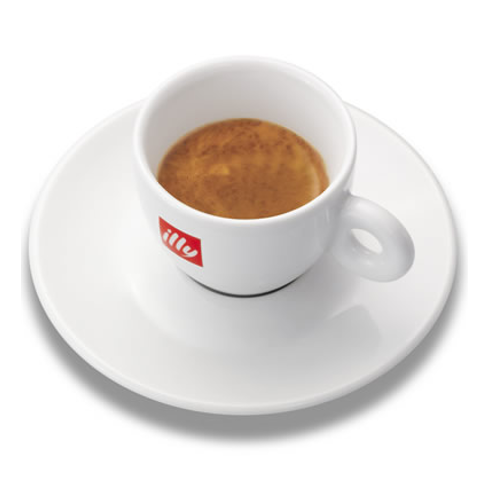
\includegraphics[width=0.2\textwidth]{img/conclusion/espresso_tmp}}
	\only<2->{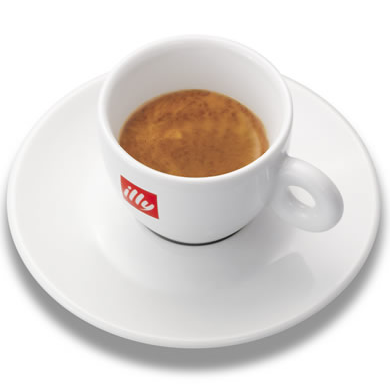
\includegraphics[width=0.2\textwidth]{img/conclusion/espresso}}
	\only<-2>{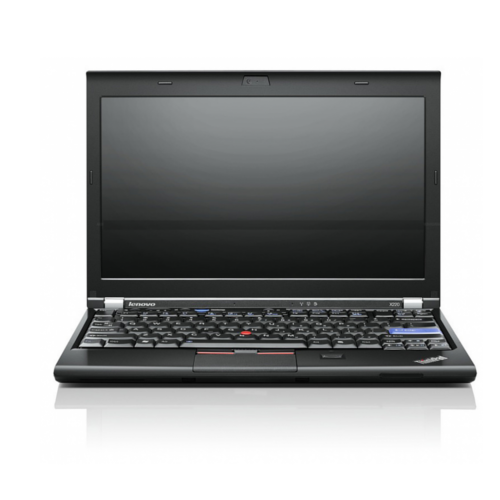
\includegraphics[width=0.2\textwidth]{img/conclusion/ordi_tmp}}
	\only<3->{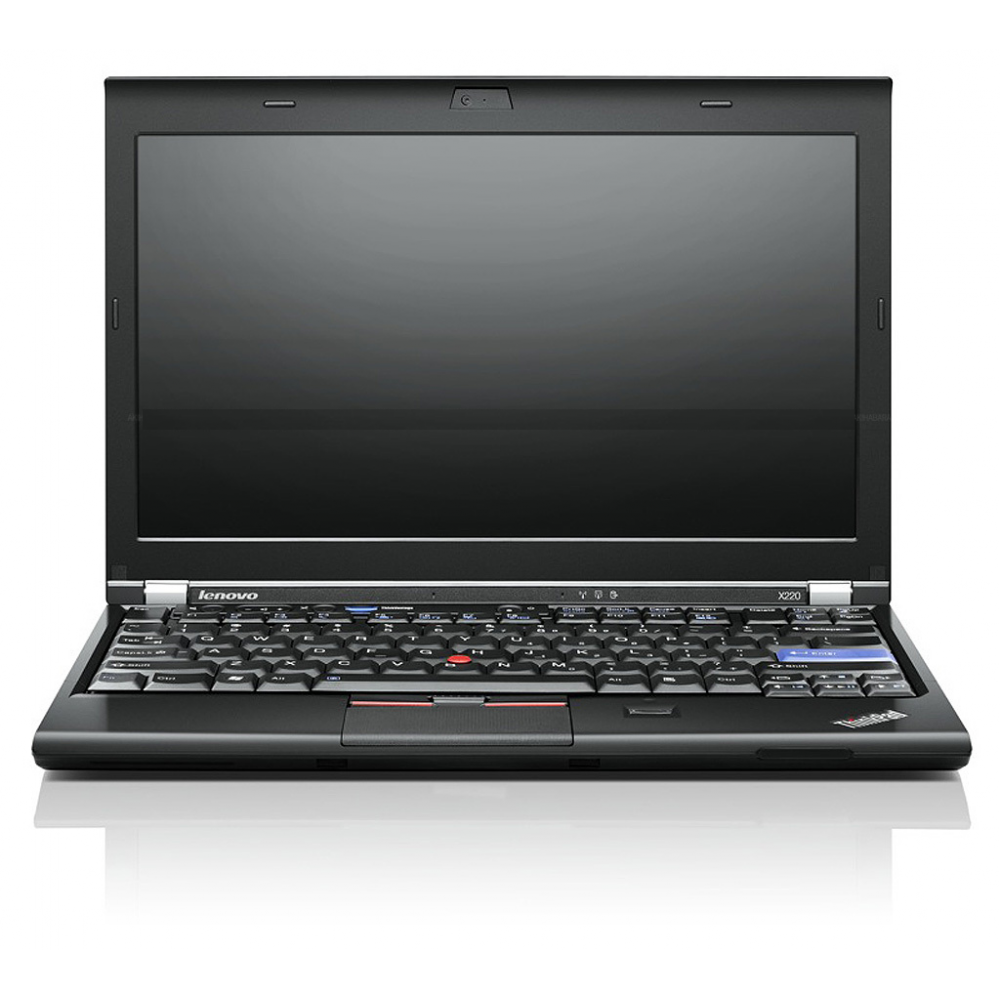
\includegraphics[width=0.2\textwidth]{img/conclusion/ordi}}
\end{center}
\begin{center}
	\only<4>{
\includegraphics[width=0.3\textwidth]{img/conclusion/cafe_renverse_tmp}}
	\only<5->{
\includegraphics[width=0.3\textwidth]{img/conclusion/cafe_renverse}}
\end{center}
\end{block}
\end{frame}

\section*{Questions \& Démo}
\begin{frame}{Merci pour votre attention}{Questions \& Démo}
\vspace*{\stretch{1}}
\texttt{https://github.com/cogitoTeam/artificial\_consciousness}
\end{frame}

\end{document}